\documentclass[12pt, openany, oneside]{book}

\usepackage{listings}
\usepackage[dvipsnames]{xcolor}
\usepackage{ctex}
\usepackage{fontspec}
\usepackage{setspace}
\usepackage{tikz}
\usepackage{anyfontsize}
\usepackage{sectsty}
\usepackage{titlesec}
\usepackage{float}
\usepackage[hidelinks]{hyperref}
\usepackage[a4paper]{geometry}
\usepackage{url}
\usepackage{amssymb}
\usepackage{fontawesome5}
\usepackage[most]{tcolorbox}
\usepackage{stackengine}
\usepackage{multirow}
\usepackage[T1]{fontenc}
\usepackage{diagbox}
\usepackage{longtable}
\usepackage{newtxtt}
\usepackage{pgf-umlcd}
\usepackage{bbding}
\usepackage[edges]{forest}
\usepackage{amsmath}
\usepackage{algorithm}
\usepackage{algpseudocode}
% \usepackage{minted}

\usetikzlibrary{calc,trees,positioning,arrows,fit,shapes}
\usetikzlibrary{shapes.multipart,chains}
\usetikzlibrary{shadows}
\usetikzlibrary{arrows.meta}
\usetikzlibrary{matrix,backgrounds}

\tikzstyle{ptr}  = [draw, -{Stealth[scale=1.0]}, blue]
\tikzstyle{head} = [rectangle, draw, text height=3mm, text width=3mm,
                    text centered, node distance=3cm, inner sep=0pt]
\tikzstyle{data} = [rectangle split, rectangle split parts=2, draw,
                    text centered, minimum height=3em]
\newcommand{\data}{
  data \nodepart{second}
  \phantom{\texttt{NULL}}
}

\def\x{0}
\def\y{0}
\def\k{0}
\def\radius{5}

\makeatletter
\newcommand{\verbatimfont}[1]{\renewcommand{\verbatim@font}{\ttfamily#1}}
\makeatother

\makeatletter
\def\BState{\State\hskip-\ALG@thistlm}
\makeatother

\tikzstyle{startend} = [rectangle, rounded corners, minimum width=3cm, minimum height=1cm, text centered, draw=black, fill=red!30]
\tikzstyle{io}        = [trapezium, trapezium left angle=70, trapezium right angle=110, minimum width=3cm, inner xsep = -15pt, minimum height=1cm, text centered, draw=black, fill=blue!30]
\tikzstyle{process}   = [rectangle, minimum width=3cm, minimum height=1cm, inner ysep=0, text centered, draw=black, fill=orange!30]
\tikzstyle{decision}  = [diamond,shape aspect=2.5, minimum width=3cm, minimum height=1cm, inner xsep=0,text centered, draw=black, fill=green!30]
\tikzstyle{arrow}     = [thick,->,>=stealth]

\def\rlwd{.5pt} \def\rlht{2.2ex} \def\rldp{.5ex}
\def\mydiv#1{~%
  \rule[-\rldp]{\rlwd}{\rlht}%
  \setbox0=\hbox{~#1}%
  \stackunder[\dimexpr\rldp-\rlwd]{~#1}{\rule{\wd0}{\rlwd}}%
}

\definecolor{mycolor}{RGB}{0,128,128}
\newtcbox{\mybox} {
    on line,
    colback=mycolor,
    fontupper=\bfseries\color{white},
    boxrule=0pt,
    arc=5pt, 
    boxsep=0pt, 
    left=2pt, 
    right=2pt, 
    top=5pt, 
    bottom=5pt
}

\setstretch{1.5}
\setlength{\parindent}{0cm}

\geometry{a4paper,top=2.5cm,bottom=2.5cm}

\titleformat{\chapter}{\Huge\Huge\bfseries}{\chaptertitlename\ \thechapter{\ }}{0pt}{\Huge}{}
\titlespacing{\chapter}{0pt}{0pt}{12pt}

\definecolor{dkgreen}{rgb}{0,0.4,0}
\definecolor{gray}{rgb}{0.5,0.5,0.5}
\definecolor{mauve}{rgb}{0.58,0,0.82}
\definecolor{LightGray}{gray}{0.9}

\lstset{
    basicstyle=\linespread{1.3} \fontspec{Consolas},    %  the size of the fonts that are used for the code
	basewidth=0.5em,
    numbers=left,            % where to put the line-numbers
    numberstyle=\color{black},  % the style that is used for the line-numbers
    numbersep=10pt,                  % how far the line-numbers are from the code
    backgroundcolor=\color{white},
    showspaces=false,
    showstringspaces=false,
    showtabs=false,
    frame=single,                   % adds a frame around the code
    rulecolor=\color{black},        % if not set, the frame-color may be changed on line-breaks within not-black text (e.g. commens (green here))
    tabsize=4,                      % sets default tabsize to 2 spaces
    captionpos=t,                   % sets the caption-position to bottom
    breaklines=false,                % sets automatic line breaking
    breakatwhitespace=true,        % sets if automatic breaks should only happen at whitespace
    title=\lstname,                   % show the filename of files included with \lstinputlisting;
    % also try caption instead of title
    numberstyle=\color{black},		% line number color
    keywordstyle=\color{blue},          % keyword style
    commentstyle=\color{dkgreen},       % comment style
    stringstyle=\color{mauve},         % string literal style
    escapeinside={\%*}{*)},            % if you want to add LaTeX within your code
    morekeywords={*,...}               % if you want to add more keywords to the set
}

\begin{document}

\pagestyle{plain}

\begin{tikzpicture}[overlay,remember picture]
	% Background color
	\fill[
		black!2]
	(current page.south west) rectangle (current page.north east);

	% Rectangles
	\shade[
		left color=Dandelion,
		right color=Dandelion!40,
		transform canvas ={rotate around ={45:($(current page.north west)+(0,-6)$)}}]
	($(current page.north west)+(0,-6)$) rectangle ++(9,1.5);

	\shade[
		left color=lightgray,
		right color=lightgray!50,
		rounded corners=0.75cm,
		transform canvas ={rotate around ={45:($(current page.north west)+(.5,-10)$)}}]
	($(current page.north west)+(0.5,-10)$) rectangle ++(15,1.5);

	\shade[
		left color=lightgray,
		rounded corners=0.3cm,
		transform canvas ={rotate around ={45:($(current page.north west)+(.5,-10)$)}}] ($(current page.north west)+(1.5,-9.55)$) rectangle ++(7,.6);

	\shade[
		left color=orange!80,
		right color=orange!60,
		rounded corners=0.4cm,
		transform canvas ={rotate around ={45:($(current page.north)+(-1.5,-3)$)}}]
	($(current page.north)+(-1.5,-3)$) rectangle ++(9,0.8);

	\shade[
		left color=red!80,
		right color=red!80,
		rounded corners=0.9cm,
		transform canvas ={rotate around ={45:($(current page.north)+(-3,-8)$)}}] ($(current page.north)+(-3,-8)$) rectangle ++(15,1.8);

	\shade[
		left color=orange,
		right color=Dandelion,
		rounded corners=0.9cm,
		transform canvas ={rotate around ={45:($(current page.north west)+(4,-15.5)$)}}]
	($(current page.north west)+(4,-15.5)$) rectangle ++(30,1.8);

	\shade[
		left color=RoyalBlue,
		right color=Emerald,
		rounded corners=0.75cm,
		transform canvas ={rotate around ={45:($(current page.north west)+(13,-10)$)}}]
	($(current page.north west)+(13,-10)$) rectangle ++(15,1.5);

	\shade[
		left color=lightgray,
		rounded corners=0.3cm,
		transform canvas ={rotate around ={45:($(current page.north west)+(18,-8)$)}}]
	($(current page.north west)+(18,-8)$) rectangle ++(15,0.6);

	\shade[
		left color=lightgray,
		rounded corners=0.4cm,
		transform canvas ={rotate around ={45:($(current page.north west)+(19,-5.65)$)}}]
	($(current page.north west)+(19,-5.65)$) rectangle ++(15,0.8);

	\shade[
		left color=OrangeRed,
		right color=red!80,
		rounded corners=0.6cm,
		transform canvas ={rotate around ={45:($(current page.north west)+(20,-9)$)}}]
	($(current page.north west)+(20,-9)$) rectangle ++(14,1.2);

	% Year
	% \draw[ultra thick,gray]
	% ($(current page.center)+(5,2)$) -- ++(0,-3cm)
	node[
			midway,
			left=0.25cm,
			text width=5cm,
			align=right,
			black!75
		]
		{
			% {\fontsize{25}{30} \selectfont \bf ANNUAL \\[10pt] REPORT}
		}
	node[
			midway,
			right=0.25cm,
			text width=6cm,
			align=left,
			orange]
		{
			% {\fontsize{72}{86.4} \selectfont 2020}
		};

	% Title
	\node[align=center] at ($(current page.center)+(0,-6)$)
	{
	{\fontsize{60}{60} \selectfont {{数据结构与算法}}} \\[1cm]
	{\fontsize{40}{40} \selectfont {{Data Structure and Algorithm}}} \\[2cm]
	{\fontsize{20}{19.2} \selectfont \textcolor{orange}{ \bf 极夜酱}} \\[4pt]
	};
\end{tikzpicture}

\newpage

\setcounter{tocdepth}{1}
\tableofcontents
\thispagestyle{empty}

\newpage

\setcounter{page}{1}

\part{基础篇}

% \chapter{数据结构与算法}

\section{算法}

\subsection{算法(Algorithm)}

算法是一个很古老的概念,最早来自数学领域。 \\

有一个关于算法的小故事:在很久很久以前,曾经有一个顽皮又聪明的熊孩子,天天在课堂上调皮捣蛋。终于有一天,老师忍无可忍,对熊孩子说:“臭小子,你又调皮啊!今天罚你做加法,算出$ 1 + 2 + 3 + \dots + 9999 + 10000 $累加的结果,算不完不许回家!”  \\

老师以为,熊孩子会按部就班地一步一步计算:

\vspace{-1cm}

\begin{align*}
	1 + 2  & = 3  \\
	3 + 3  & = 6  \\
	6 + 4  & = 10 \\
	10 + 5 & = 15 \\
	\dots
\end{align*}

这还不得算到明天天亮?够这小子受的!老师心里幸灾乐祸地想着。谁知仅仅几分钟后…… \\

“老师,我算完了!结果是50005000,对不对?” \\

“这,这,这……你小子怎么算得这么快?我读书多,你骗不了我的!” \\

看着老师惊讶的表情,熊孩子微微一笑,讲出了他的计算方法。 \\

首先把从1到10000这10000个数字两两分组相加:

\vspace{-1cm}

\begin{align*}
	1 + 10000 & = 10001 \\
	2 + 9999  & = 10001 \\
	3 + 9998  & = 10001 \\
	4 + 9997  & = 10001 \\
	\dots
\end{align*}

一共有$ 10000 \div 2 = 5000 $组,所以1到10000相加的总和可以这样来计算:

$$
	(1 + 10000) \times 10000 \div 2 = 50005000
$$

这个熊孩子就是后来著名的犹太数学家约翰·卡尔·弗里德里希·高斯,而他所采用的这种等差数列求和的方法,被称为高斯算法。 \\

算法是解决问题的一种方法或一个过程,是一个由若干运算或指令组成的有穷序列。求解问题的算法可以看作是输入实例与输出之间的函数。 \\

算法有5个特点:

\begin{enumerate}
	\item 有穷性(finiteness):算法必须能在执行有限个步骤之后终止。
	\item 确定性(definiteness):算法的每一步骤必须有确切的定义。
	\item 输入项(input):一个算法有0个或多个输入。
	\item 输出项(output):一个算法有一个或多个输出,没有输出的算法是毫无意义的。
	\item 可行性(effectiveness):算法中执行的任何计算步骤都是可以被分解为基本的可执行的操作步。
\end{enumerate}

\subsection{算法描述}

算法是可完成特定任务的一系列步骤,算法的计算过程定义明确,通过一些值作为输入并产生一些值作为输出。 \\

流程图(flow chart)是算法的一种图形化表示方式,使用一组预定义的符号来说明如何执行特定任务。

\begin{itemize}
	\item 圆角矩形:开始和结束
	\item 矩形:数据处理
	\item 平行四边形:输入/输出
	\item 菱形:分支判断条件
	\item 流程线:步骤
\end{itemize}

\begin{figure}[H]
	\centering
	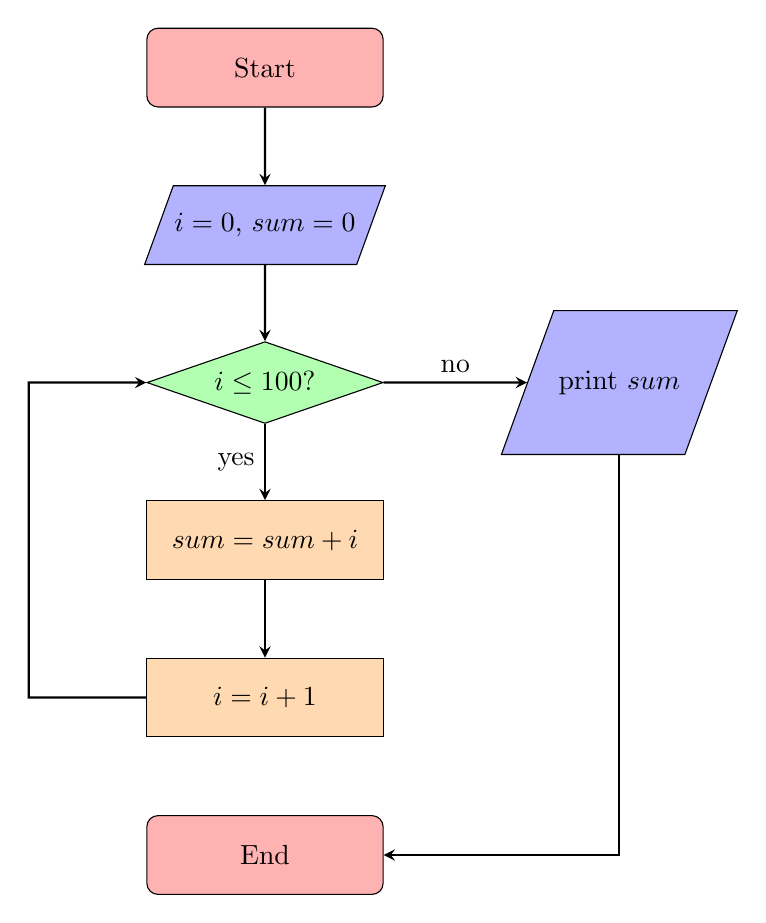
\begin{tikzpicture}[node distance=2cm]
		\node (start) [startend] {Start};
		\node (init)   [io, below of=start] {$ i = 0 $, $ sum = 0 $};
		\node (decision)  [decision, below of=init] {$ i \le 100 $?};
		\node (accumulation) [process, below of=decision] {$ sum = sum + i $};
		\node (update) [process, below of=accumulation] {$ i = i + 1 $};
		\node (output) [io, right of=decision, xshift=2.5cm] {print $ sum $};
		\node (end) [startend, below of=update] {End};

		\draw [arrow] (start) -- (init);
		\draw [arrow] (init) -- (decision);
		\draw [arrow] (decision) -- node[anchor=east] {yes } (accumulation);
		\draw [arrow] (accumulation) -- (update);
		\draw [arrow] (update) -- (-3,-8) -- (-3,-4) -- (decision);
		\draw [arrow] (decision) -- node[anchor=south] {no} (output);
		\draw [arrow] (output) |- (end);
	\end{tikzpicture}
	\caption{计算$ \sum_{i=1}^{100} i $的流程图}
\end{figure}

伪代码(pseudocode)是一种非正式的,类似于英语结构的,用于描述模块结构图的语言。使用伪代码的目的是使被描述的算法可以容易地以任何一种编程语言实现。

\begin{algorithm}[H]
	\caption{插入排序}
	\begin{algorithmic}[1]
		\Procedure{insertionSort}{A[0..n-1]}
		\For {j = 2 to n - 1}
		\State key = A[j]
		\State i = j - 1
		\While {i > 0 and A[i] > key}
		\State A[i+1] = A[i]
		\State i = i - 1
		\EndWhile
		\State A[i+1] = key
		\EndFor
		\State \Return A
		\EndProcedure
	\end{algorithmic}
\end{algorithm}

\newpage

\section{算法效率}

\subsection{算法效率}

算法有高效的,也有拙劣的。在高斯的故事中,高斯所用的算法显然是更加高效的算法,它利用等差数列的规律,四两拨千斤,省时省力地求出了最终结果。而老师心中所想的算法,按部就班地一个数一个数进行累加,则是一种低效、笨拙的算法。虽然这种算法也能得到最终结果,但是其计算过程要低效得多。 \\

在计算机领域,我们同样会遇到各种高效和拙劣的算法。衡量算法好坏的重要标准有两个:时间复杂度、空间复杂度。 \\

让我们来想象一个场景:某一天,小灰和大黄同时加入了同一家公司。老板让他们完成一个需求。一天后,小灰和大黄交付了各自的代码,两人的代码实现的功能差不多。但是,大黄的代码运行一次要花100 ms,占用内存5 MB;小灰的代码运行一次要花100 s,占用内存500 MB。 \\

“小灰,收拾东西走人,明天不用来上班了!” \\

小灰虽然也按照老板的要求实现了功能,但他的代码存在两个很严重的问题:运行时间长、占用空间大。 \\

算法效率分析指的是算法求解一个问题所需要的时间资源和空间资源。效率可以通过对算法执行基本运算(步数)的数目进行估算,度量一个算法运算时间的三种方式:

\begin{itemize}
	\item 最好情形时间复杂度
	\item 最坏情形时间复杂度
	\item 平均情形时间复杂度
\end{itemize}

最坏情形是任何规模为n的问题实例运行时间的上界,即任何规模为n的实例,其运行时间都不会超过最坏情况的运行时间。 \\

对某些算法,最坏情况经常发生。例如在某个数据库中查询不存在的某条诗句就是查询算法的最坏情形。平均情形有时跟最坏情形差不多。

\subsection{时间复杂度(Time Complexity)}

算法的效率主要取决于算法本身,与计算模型(例如计算机)无关,这样可以通过分析算法的运行时间从而比较出算法之间的快慢。分析一个算法的运行时间应该主要关注与问题规模有关的主要项,其它低阶项,甚至主要项的常数系数都可以忽略。 \\

渐进时间复杂度用大写$ O $来表示,所以也被称为大$ O $表示法。

时间复杂度有如下原则:

\begin{enumerate}
	\item 如果运行时间是常数量级,则用$ O(1) $表示。
	\item 只保留时间函数中的最高阶项。
	\item 如果最高阶项存在,则省去最高阶项前面的系数。
\end{enumerate}

在编程的世界中有各种各样的算法,有许多不同形式的时间复杂度,例如:$ O(1) $、$ O(logn) $、$ O(n) $、$ O(nlogn) $、$ O(n^2) $、$ O(2^n) $、$ O(n!) $等。

\subsection{空间复杂度(Space Complexity)}

内存空间是有限的,在时间复杂度相同的情况下,算法占用的内存空间自然是越小越好。如何描述一个算法占用的内存空间的大小呢?这就用到了算法的另一个重要指标——空间复杂度。 \\

和时间复杂度类似,空间复杂度是对一个算法在运行过程中临时占用存储空间大小的量度,它同样使用了大$ O $表示法。 \\

正所谓鱼和熊掌不可兼得,很多时候,我们不得不在时间复杂度和空间复杂度之间进行取舍。在绝大多数时候,时间复杂度更为重要一些,我们宁可多分配一些内存空间,也要提升程序的执行速度。

\newpage

\section{基础算法}

\subsection{暴力枚举}

暴力破解法也称穷举法,思想就是列举出所有可能情况,然后根据条件判断此答案是否合适,合适就保留,不合适就丢弃。暴力法主要利用计算机运算速度快、精确度高的特点。因此暴力法是通过牺牲时间来换取答案的全面性。 \\

\mybox{鸡兔同笼} \\

上有三十五头,下有九十四足,问鸡兔各几何?

\begin{lstlisting}[language=C]
void count(int head, int foot) {
	for(int chicken = 0; chicken <= head; chicken++) {
		int rabbit = head - chicken;
		if(chicken*2 + rabbit*4 == foot) {
			printf("鸡:%2d\t兔:%2d\n", chicken, rabbit);
		}
	}
}
\end{lstlisting}

\vspace{0.5cm}

\mybox{百钱买百鸡} \\

公鸡5文钱1只,母鸡3文钱1只,小鸡1文钱3只,如果用100文钱买100只鸡,那么公鸡、母鸡和小鸡各应该买多少只?

\begin{lstlisting}[language=C]
void buy(int n, int money) {
	for(int x = 0; x <= n/5; x++) {
		for(int y = 0; y <= n/3; y++) {
			int z = n - x - y;
			if(z > 0 && z % 3 == 0 && 5*x + 3*y + z/3 == money) {
				printf("公鸡:%3d\t母鸡:%3d\t小鸡:%3d\n", x, y, z);
			}
		}
	}
}
\end{lstlisting}

\subsection{字符串逆序}

将一个字符串中的字符顺序颠倒过来实现逆序。 \\

\mybox{字符串逆序}

\begin{lstlisting}[language=C]
void reverse(char *str) {
	int i = 0;
	int j = strlen(str) - 1;
	while(i < j) {
		char temp = str[i];
		str[i] = str[j];
		str[j] = temp;
		i++;
		j--;
	}
}
\end{lstlisting}

\subsection{随机算法}

随机算法就是在算法中引入随机因素,通过随机数选择算法的下一步操作,它采用了一定程序的随机性作为其逻辑的一部分。 \\

只有随机数生成器的情况下如何计算圆周率的近似值?蒙特卡洛算法就是一种随机算法,用于近似计算圆周率$ \pi $的值。 \\

蒙特卡洛算法是以概率和统计理论方法为基础的一种计算方法,将所求解的问题同一定的概率模型相联系,用电子计算机实现统计模拟或抽样,以获得问题的近似解。为象征性地表明这一方法的概率统计特征,故借用赌城蒙特卡罗命名。 \\

蒙特卡洛算法的基本思想就是当样本数量足够大时,可以用频率去估计概率,这也是求圆周率$ \pi $的常用方法。

\begin{figure}[H]
	\centering
	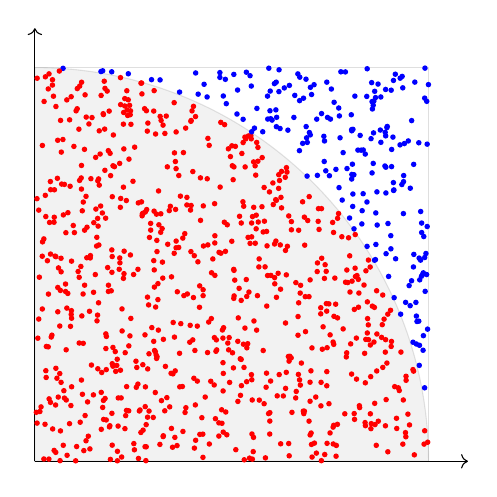
\begin{tikzpicture}
		\draw[fill=gray, opacity=0.1] (\radius,0) arc(0:90:\radius) -- (0,0) -- cycle;
		\draw[gray, opacity=0.25] (0,0) rectangle (\radius,\radius);
		\draw[->] (0,0) -- (1.1*\radius,0);
		\draw[->] (0,0) -- (0,1.1*\radius);
		\foreach \i in {1,2,...,1000}{
				\typeout{Point \i}
				\pgfmathsetmacro\x{\radius*rnd}
				\typeout{X \x}
				\pgfmathsetmacro\y{\radius*rnd}
				\typeout{Y \y}
				\pgfmathsetmacro\k{(pow(\x,2)+pow(\y,2)) <pow(\radius,2)}
				\typeout{im Kreis?: \k}
				\pgfmathparse{ifthenelse(\k==1,"red","blue")}
				\fill[\pgfmathresult] (\x,\y)circle(1pt);
			}
	\end{tikzpicture}
	\caption{蒙特卡洛算法}
\end{figure}


当在$ [0, 1] $的范围内随机选择一个坐标$ (x, y) $时,每个坐标点被选中的概率相等,则坐标落在直径为1的正方形中的圆的概率为:

$$
	P \left( \sqrt{x^2 + y^2} \le 1 \right) = {\pi \over 4}
$$

在生成大量随机点的前提下能得到尽可能接近圆周率的值。 \\

\mybox{蒙特卡罗算法}

\begin{lstlisting}[language=C]
double montePI(int n) {
	int cnt = 0;        // 圆内点的数量
	for(int i = 0; i < n; i++) {
		double x = rand() / (RAND_MAX + 1.0);   // [0, 1]
		double y = rand() / (RAND_MAX + 1.0);   // [0, 1]
		if(sqrt(x*x + y*y) <= 1) {
			cnt++;
		}
	}
	return 4.0 * cnt / n;
}
\end{lstlisting}

\newpage

\section{数据结构}

\subsection{数据结构(Data Structure)}

数据结构是算法基石,是计算机数据的组织、管理和存储的方式,数据结构指的是相互之间存在一种或多种特定关系的数据元素的集合。一个好的数据结构可以带来更高的运行或者存储效率。 \\

\begin{figure}[H]
	\centering
	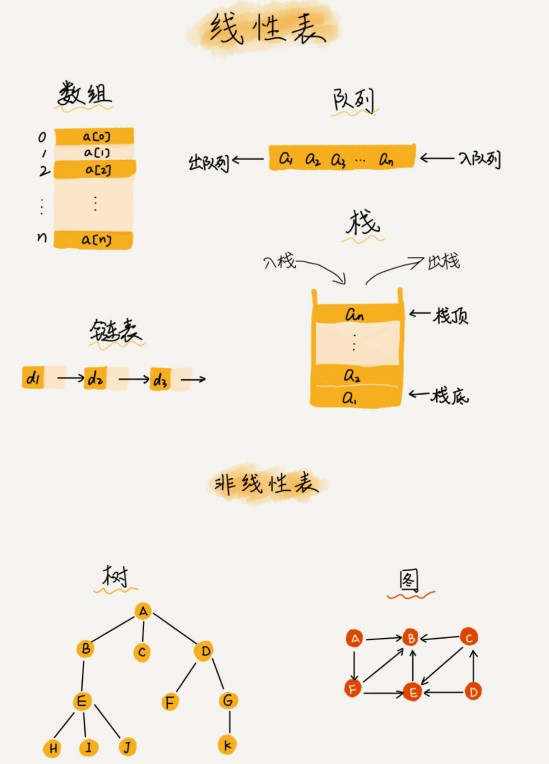
\includegraphics[]{img/C1/1-4/1.png}
	\caption{常用数据结构}
\end{figure}

\newpage
% \chapter{数组}

\section{数组}

\subsection{数组(Array)}

数组是数据结构中最简单的结构,很多编程语言都内置数组。数组是有限个相同类型的变量所组成的集合,数组中的每一个变量被称为元素。\\

创建数组时会在内存中划分出一块连续的内存,将数据按顺序进行存储,数组中的每一个元素都有着自己的下标(index),下标从0开始一直到数组长度-1。因为数组在存储数据时是按顺序存储的,存储数据的内存也是连续的。\\

对于数组来说,读取元素是最简单的操作。由于数组在内存中顺序存储,所以只要给出数组的下标,就可以读取到对应位置的元素。像这种根据下标读取元素的方式叫作随机读取。但是需要注意的是,数组的下标范围必须在0到数组长度-1之内,否则会出现数组越界。数组读取元素的时间复杂度是$ O(1) $。\\

数组拥有非常高效的随机访问能力,只要给出下标,就可以用常量时间找到对应元素。有一种高效查找元素的算法叫作二分查找,就是利用了数组的这个优势。\\

数组的劣势体现在插入和删除元素方面。由于数组元素连续紧密地存储在内存中,插入、删除元素都会导致大量元素被迫移动,影响效率。总的来说,数组所适合的是读操作多、写操作少的场景。\\

\mybox{更新数组元素}

\begin{lstlisting}[language=Python]
arr = [3, 1, 2, 5, 4, 9, 7, 2]
arr[5] = 10
print(arr[5])
\end{lstlisting}

\newpage

\section{查找算法}

\subsection{顺序查找(Sequence Search)}

顺序查找也称线性查找,是一种按照序列原有顺序进行遍历比较查询的基本查找算法。\\

对于任意一个序列以及一个需要查找的元素(关键字),将关键字与序列中元素依次比较,直到找出与给定关键字相同的元素,或者将序列中的元素与其都比较完为止。若某个元素的值与关键字相等,则查找成功;如果直到最后一个元素,元素的值和关键字比较都不等时,则查找不成功。\\

最好的情况就是在第一个位置就找到,算法时间复杂度为$ O(1) $。\\

最坏情况是关键字不存在,需要进行$ n $次比较,时间复杂度为$ O(n) $。\\

平均查找次数为$ (n + 1) / 2 $,平均时间复杂度为$ O(n) $。\\

\mybox{顺序查找}

\begin{lstlisting}[language=C]
int sequence_search(int *arr, int n, int key) {
    for (int i = 0; i < n; i++) {
        if (arr[i] == key) {
            return i;
        }
    }
    return -1;
}
\end{lstlisting}

\vspace{0.5cm}

\subsection{二分查找(Binary Search)}

二分查找法也称折半查找,是一种效率较高的查找方法。折半查找要求线性表必须采用顺序存储结构,而且表中元素按关键字有序排列。\\

算法思想是假设表中元素是按升序排列,将表中间位置的关键字与查找关键字比较,如果两者相等,则查找成功;否则利用中间位置记录将表分成前、后两个子表,如果中间位置的关键字大于查找关键字,则进一步查找前一子表,否则进一步查找后一子表。重复以上过程,直到找到满足条件的记录,使查找成功,或直到子表不存在为止,此时查找不成功。\\

二分查找法的时间复杂度为$ O(logn) $。\\

\mybox{二分查找}

\begin{lstlisting}[language=C]
int binary_search(int *arr, int n, int key) {
    int start = 0;
    int end = n - 1;
    while (start <= end) {
        int mid = (start + end) / 2;
        if (arr[mid] == key) {
            return mid;
        } else if (arr[mid] < key) {
            start = mid + 1;
        } else {
            end = mid - 1;
        }
    }
    return -1;
}
\end{lstlisting}

\newpage

\section{数组元素插入与删除}

\subsection{插入元素}

在数组中插入元素存在3种情况:

\begin{figure}[H]
	\centering
	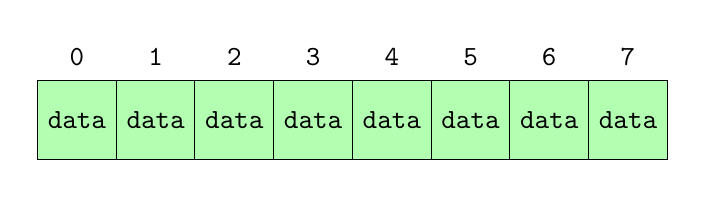
\begin{tikzpicture}[font=\ttfamily,
			array/.style={matrix of nodes,nodes={draw, minimum size=10mm, fill=green!30},column sep=-\pgflinewidth, row sep=0.5mm, nodes in empty cells,
					row 1/.style={nodes={draw=none, fill=none, minimum size=5mm}},
				}]

		\matrix[array] (array) {
			0    & 1    & 2    & 3    & 4    & 5    & 6    & 7    \\
			data & data & data & data & data & data & data & data \\
		};
	\end{tikzpicture}
	\caption{数组}
\end{figure}

\subsubsection{尾部插入}

直接把插入的元素放在数组尾部的空闲位置即可。

\subsubsection{中间插入}

首先把插入位置及后面的元素向后移动,腾出位置,再把要插入的元素放入该位置上。\\

\mybox{插入元素}

\begin{lstlisting}[language=C]
int insert(int *arr, int n, int index, int val) {
    if(index < 0 || index >= n) {
        return n;
    }
    for(int i = n - 1; i >= index; i--) {
        arr[i+1] = arr[i];
    }
    arr[index] = val;
    n++;
    return n;
}
\end{lstlisting}

\subsubsection{超范围插入}

数组的长度在创建时就已经确定了,要实现数组的扩容,只能创建一个新数组,长度是旧数组的2倍,再把旧数组中的元素全部复制过去,这样就实现了数组的扩容。\\

数组插入元素最好情况是尾部插入,无需移动任何元素,时间复杂度为$ O(1) $。最坏情况是在第一个位置插入,这样就需要移动后面所有$ n - 1 $个元素,时间复杂度为$ O(n) $。因此,总体的时间复杂度为$ O(n) $。\\

\subsection{删除元素}

数组的删除操作与插入操作过程相反,如果被删除的元素位于数组中间,其后的元素都需要向前挪动一位。\\

\mybox{删除元素}

\begin{lstlisting}[language=C]
int delete(int *arr, int n, int index) {
    if(index < 0 || index >= n) {
        return n;
    }
    for(int i = index + 1; i < n; i++) {
        arr[i-1] = arr[i];
    }
    n--;
    return n;
}
\end{lstlisting}

数组的删除操作,由于只涉及元素的移动,时间复杂度为$ O(n) $。\\

对于删除操作,其实还存在一种取巧的方式,前提是数组元素没有顺序要求。如需要删除数组中某个元素,可直接把最后一个元素复制到被删除元素的位置,然后再删除最后一个元素。这样一来,无须进行大量的元素移动,时间复杂度降低为$ O(1) $。当然,这种方式只作参考,并不是删除元素主流的操作方式。

\newpage
% \chapter{链表}

\section{链表}

\subsection{单向链表(Singly Linked List)}

为避免元素的移动,采用线性表的另一种存储方式:链式存储结构。链表是一种在物理上非连续、非顺序的数据结构,由若干结点(node)所组成。 \\

单向链表的每一个结点又包含两部分,一部分是存放数据的数据域data,另一部分是指向下一个结点的指针域next。结点可以在运行时动态生成。

\vspace{-0.5cm}

\begin{lstlisting}[language=C]
typedef struct Node {
    dataType data;          // 数据域
    struct Node *next;		// 指针域
} Node;
\end{lstlisting}

链表的第一个结点被称为头结点,最后一个节点被称为尾结点,尾结点的next指针指向空NULL。 \\

\begin{figure}[H]
	\centering
	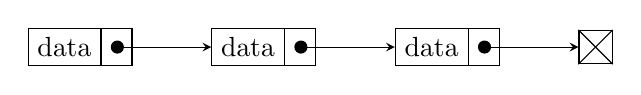
\begin{tikzpicture}[list/.style={rectangle split, rectangle split parts=2,
					draw, rectangle split horizontal}, >=stealth, start chain]
		\node[list,on chain] (A) {data};
		\node[list,on chain] (B) {data};
		\node[list,on chain] (C) {data};
		\node[on chain,draw,inner sep=6pt] (D) {};
		\draw (D.north east) -- (D.south west);
		\draw (D.north west) -- (D.south east);
		\draw[*->] let \p1 = (A.two), \p2 = (A.center) in (\x1,\y2) -- (B);
		\draw[*->] let \p1 = (B.two), \p2 = (B.center) in (\x1,\y2) -- (C);
		\draw[*->] let \p1 = (C.two), \p2 = (C.center) in (\x1,\y2) -- (D);
	\end{tikzpicture}
	\caption{单向链表}
\end{figure}

与数组按照下标来随机寻找元素不同,对于链表的其中一个结点A,只能根据结点A的next指针来找到该结点的下一个结点B,再根据结点B的next指针找到下一个节点C…… \\

数组在内存中的存储方式是顺序存储,链表在内存中的存储方式则是随机存储。链表采用了见缝插针的方式,每一个结点分布在内存的不同位置,依靠next指针关联起来。这样可以灵活有效地利用零散的碎片空间。

\subsection{双向链表(Doubly Linked List)}

那么,通过链表的一个结点,如何能快速找到它的前一个结点呢?要想让每个结点都能回溯到它的前置结点,可以使用双向链表。 \\

双向链表比单向链表稍微复杂一点,它的每一个结点除了拥有data和next指针,还拥有指向前置结点的prev指针。 \\

\begin{figure}[H]
	\centering
	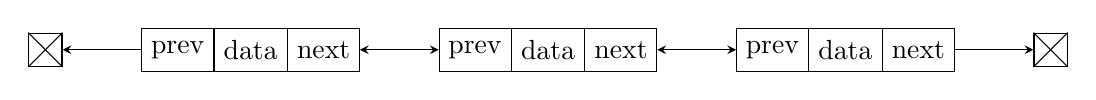
\begin{tikzpicture}[list/.style={rectangle split, rectangle split parts=3,
					draw, rectangle split horizontal}, >=stealth, start chain]
		\node[on chain,draw,inner sep=6pt] (NULL1) {};
		\node[list,on chain] (A) {prev \nodepart{second} data \nodepart{third} next};
		\node[list,on chain] (B) {prev \nodepart{second} data \nodepart{third} next};
		\node[list,on chain] (C) {prev \nodepart{second} data \nodepart{third} next};
		\node[on chain,draw,inner sep=6pt] (NULL2) {};
		\draw (NULL1.north east) -- (NULL1.south west);
		\draw (NULL1.north west) -- (NULL1.south east);
		\draw (NULL2.north east) -- (NULL2.south west);
		\draw (NULL2.north west) -- (NULL2.south east);
		\draw[<-] let \p1 = (A.west), \p2 = (A.center) in (NULL1) -- (\x1,\y2);
		\draw[<->] let \p1 = (A.east), \p2 = (A.center) in (\x1,\y2) -- (B);
		\draw[<->] let \p1 = (B.east), \p2 = (B.center) in (\x1,\y2) -- (C);
		\draw[->] let \p1 = (C.east), \p2 = (C.center) in (\x1,\y2) -- (NULL2);
	\end{tikzpicture}
	\caption{双向链表}
\end{figure}

单向链表只能从头到尾遍历,只能找到后继,无法找到前驱,因此遍历的时候不会死循环。而双向链表需要多分配一个指针的存储空间,每个结点有两个指针,分别指向直接前驱和直接后继。

\subsection{循环链表(Circular Linked List)}

除了单向链表和双向链表以外,还有循环链表。对于单向循环链表,尾结点的next指针指向头结点。对于双向循环链表,尾结点的next指针指向头结点,并且头结点的prev指针指向尾结点。 \\

\begin{figure}[H]
	\centering
	
\begin{tikzpicture}[
			list/.style={
					rectangle split,
					rectangle split parts=2,
					draw,
					rectangle split horizontal
				},
			dotarrow/.style={Circle-Stealth},
			start chain
		]
		\node[list,on chain] (A) {data};
		\node[list,on chain] (B) {data};
		\node[list,on chain] (C) {data};
		\draw[dotarrow] (A.two |- A.center) -- (B);
		\draw[dotarrow] (B.two |- B.center)  -- (C);
		\draw[dotarrow] (C.two |- C.center) to[out=-20,in=190,distance=4cm] (A);
	\end{tikzpicture}
	\caption{单向循环链表}
\end{figure}

\begin{figure}[H]
	\centering
	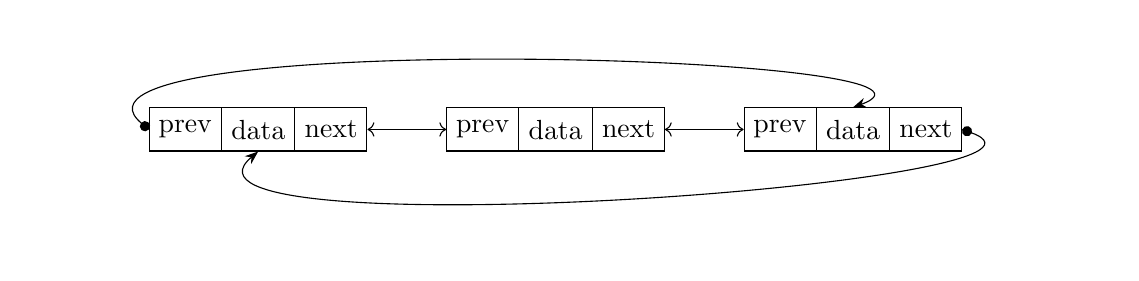
\begin{tikzpicture}[list/.style={
					rectangle split,
					rectangle split parts=3,
					draw,
					rectangle split horizontal
				},
			dotarrow/.style={Circle-Stealth},
			start chain]
		\node[list,on chain] (A) {prev \nodepart{second} data \nodepart{third} next};
		\node[list,on chain] (B) {prev \nodepart{second} data \nodepart{third} next};
		\node[list,on chain] (C) {prev \nodepart{second} data \nodepart{third} next};

		\draw[dotarrow] (A.center -| A.west) to[out=-220,in=20,distance=2cm] (C.north);
		\draw[<->] let \p1 = (A.east), \p2 = (A.center) in (\x1,\y2) -- (B);
		\draw[<->] let \p1 = (B.east), \p2 = (B.center) in (\x1,\y2) -- (C);
		\draw[dotarrow] (C.east |- C.center) to[out=-20,in=220,distance=2cm] (A.south);
	\end{tikzpicture}
	\caption{双向循环链表}
\end{figure}

\newpage

\section{链表的增删改查}

\subsection{查找结点}

在查找元素时,链表不像数组那样可以通过下标快速进行定位,只能从头结点开始向后一个一个结点逐一查找。 \\

链表中的数据只能按顺序进行访问,最坏的时间复杂度是$ O(n) $。 \\

\mybox{查找结点}

\begin{lstlisting}[language=C]
Node* search(List *head, dataType val) {
    // 查找元素位置
    Node *temp = head;
    while(temp) {
        if(temp->data == val) {
            return temp;
        }
        temp = temp->next;
    }
    return NULL;        // 未找到
}
\end{lstlisting}

\subsection{更新结点}

如果不考虑查找结点的过程,链表的更新过程会像数组那样简单,直接把旧数据替换成新数据即可。 \\

\mybox{更新结点}

\begin{lstlisting}[language=C]
void replace(List *head, int pos, dataType val) {
    // 找到元素位置
    Node *temp = head;
    for(int i = 0; i < pos; i++) {
        temp = temp->next;
    }
    temp->data = val;
}
\end{lstlisting}

\subsection{插入结点}

链表插入结点,分为3种情况:

\subsubsection{尾部插入}

把最后一个结点的next指针指向新插入的结点。

\begin{figure}[H]
	\centering
	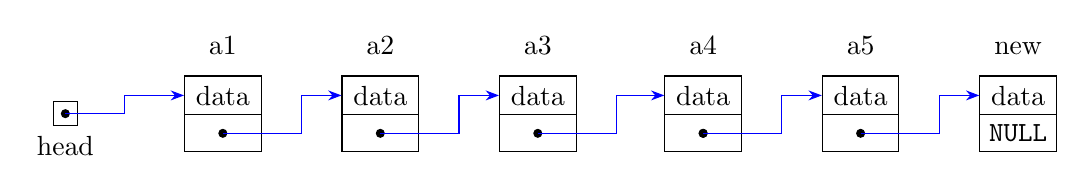
\begin{tikzpicture}[node distance=2cm, auto, scale=1,
			every node/.style={scale=1}]
		\node[head, label=below:head] (head) {};
		\node[data, right of=head] (A) {\data};
		\node[above of=A,node distance=0.5cm,label=above:a1] (a1){};
		\node[data, right of=A] (B) {\data};
		\node[above of=B,node distance=0.5cm,label=above:a2] (a2){};
		\node[data, right of=B] (C) {\data};
		\node[above of=C,node distance=0.5cm,label=above:a3] (a3){};
		\node[data, right of=C, xshift=0.1cm] (D) {\data};%, xshift=1.5cm
		\node[above of=D,node distance=0.5cm,label=above:a4] (a4){};
		\node[data, right of=D] (E) {\data};
		\node[above of=E,node distance=0.5cm,label=above:a5] (a5){};
		\node[data, right of=E] (last) {data \nodepart{second} \texttt{NULL}};
		\node[above of=last,node distance=0.5cm,label=above:new] (new){};

		\draw[fill] (head.center) circle (0.05);

		\path[ptr] (head.center) --++(right:7.5mm) |- (A.text west);
		\draw[fill] ($(A.south)!0.5!(A.text split)$) circle (0.05);
		\draw[ptr] ($(A.south)!0.5!(A.text split)$) --++(right:10mm) |- (B.text west);
		\draw[fill] ($(B.south)!0.5!(B.text split)$) circle (0.05);
		\draw[ptr] ($(B.south)!0.5!(B.text split)$) --++(right:10mm) |- (C.text west);
		\draw[fill] ($(C.south)!0.5!(C.text split)$) circle (0.05);
		\draw[ptr] ($(C.south)!0.5!(C.text split)$) --++(right:10mm) |- (D.text west);
		\draw[fill] ($(D.south)!0.5!(D.text split)$) circle (0.05);

		\draw[fill] ($(D.south)!0.5!(D.text split)$) circle (0.05);
		\draw[ptr] ($(D.south)!0.5!(D.text split)$) --++(right:10mm) |- (E.text west);
		\draw[fill] ($(E.south)!0.5!(E.text split)$) circle (0.05);
		\draw[ptr] ($(E.south)!0.5!(E.text split)$) --++(right:10mm) |- (last.text west);
	\end{tikzpicture}
	\caption{尾部插入}
\end{figure}

\subsubsection{头部插入}

先把新结点的next指针指向原先的头结点,再把新结点设置为链表的头结点。

\begin{figure}[H]
	\centering
	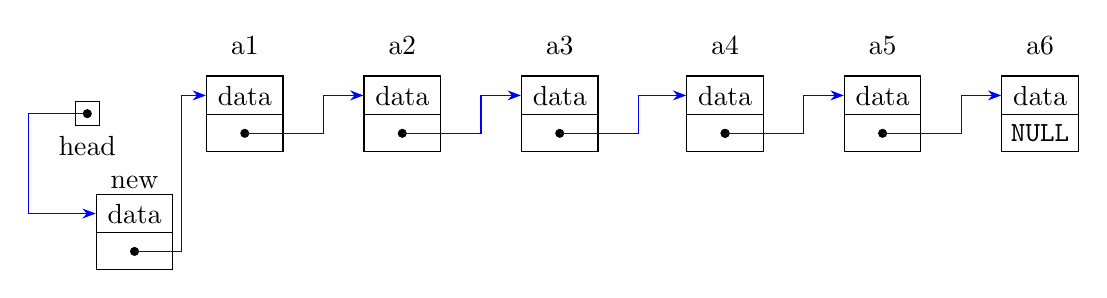
\begin{tikzpicture}[node distance=2cm, auto, scale=1,
			every node/.style={scale=1}]
		\node[head, label=below:head, xshift=-0.5cm] (head) {};
		\node[data, right of=head] (A) {\data};
		\node[above of=A,node distance=0.5cm,label=above:a1] (a1){};
		\node[data, right of=A] (B) {\data};
		\node[above of=B,node distance=0.5cm,label=above:a2] (a2){};
		\node[data, right of=B] (C) {\data};
		\node[above of=C,node distance=0.5cm,label=above:a3] (a3){};
		\node[data, below of=head, xshift=0.6cm, yshift=0.5cm] (NEW) {\data};
		\node[above of=NEW,node distance=0.3cm,label=above:new] (new){};
		\node[data, right of=C, xshift=0.1cm] (D) {\data};%, xshift=1.5cm
		\node[above of=D,node distance=0.5cm,label=above:a4] (a4){};
		\node[data, right of=D] (E) {\data};
		\node[above of=E,node distance=0.5cm,label=above:a5] (a5){};
		\node[data, right of=E] (last) {data \nodepart{second} \texttt{NULL}};
		\node[above of=last,node distance=0.5cm,label=above:a6] (a6){};

		\draw[fill] (head.center) circle (0.05);

		\path[ptr] (head.center) --++(left:7.5mm) |- (NEW.text west);
		\draw[fill] ($(NEW.south)!0.5!(NEW.text split)$) circle (0.05);
		\draw[ptr] ($(NEW.south)!0.5!(NEW.text split)$) --++(right:6mm) |- (A.text west);
		\draw[fill] ($(A.south)!0.5!(A.text split)$) circle (0.05);
		\draw[ptr] ($(A.south)!0.5!(A.text split)$) --++(right:10mm) |- (B.text west);
		\draw[fill] ($(B.south)!0.5!(B.text split)$) circle (0.05);
		\draw[ptr] ($(B.south)!0.5!(B.text split)$) --++(right:10mm) |- (C.text west);
		\draw[fill] ($(C.south)!0.5!(C.text split)$) circle (0.05);
		\draw[ptr] ($(C.south)!0.5!(C.text split)$) --++(right:10mm) |- (D.text west);
		\draw[fill] ($(D.south)!0.5!(D.text split)$) circle (0.05);
		\draw[fill] ($(D.south)!0.5!(D.text split)$) circle (0.05);
		\draw[ptr] ($(D.south)!0.5!(D.text split)$) --++(right:10mm) |- (E.text west);
		\draw[fill] ($(E.south)!0.5!(E.text split)$) circle (0.05);
		\draw[ptr] ($(E.south)!0.5!(E.text split)$) --++(right:10mm) |- (last.text west);
	\end{tikzpicture}
	\caption{头部插入}
\end{figure}

\subsubsection{中间插入}

先把新结点的next指针指向插入位置的结点,再将插入位置的前置结点的next指针指向新结点。

\begin{figure}[H]
	\centering
	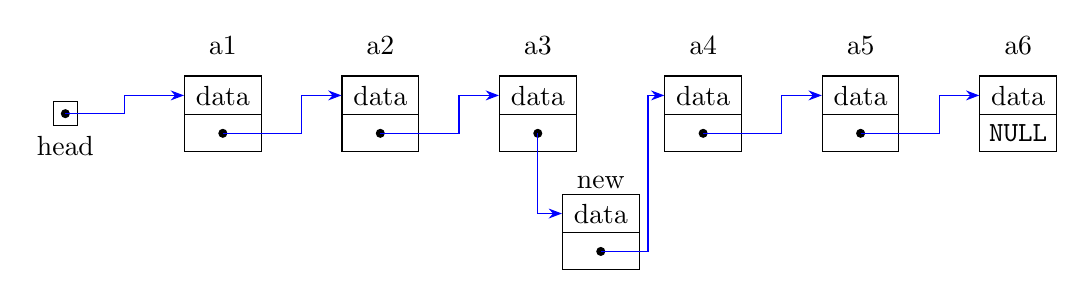
\begin{tikzpicture}[node distance=2cm, auto, scale=1,
			every node/.style={scale=1}]
		\node[head, label=below:head] (head) {};
		\node[data, right of=head] (A) {\data};
		\node[above of=A,node distance=0.5cm,label=above:a1] (a1){};
		\node[data, right of=A] (B) {\data};
		\node[above of=B,node distance=0.5cm,label=above:a2] (a2){};
		\node[data, right of=B] (C) {\data};
		\node[above of=C,node distance=0.5cm,label=above:a3] (a3){};
		\node[data, below of=C, xshift=0.8cm, yshift=0.5cm] (NEW) {\data};
		\node[above of=NEW,node distance=0.3cm,label=above:new] (new){};
		\node[data, right of=C, xshift=0.1cm] (D) {\data};%, xshift=1.5cm
		\node[above of=D,node distance=0.5cm,label=above:a4] (a4){};
		\node[data, right of=D] (E) {\data};
		\node[above of=E,node distance=0.5cm,label=above:a5] (a5){};
		\node[data, right of=E] (last) {data \nodepart{second} \texttt{NULL}};
		\node[above of=last,node distance=0.5cm,label=above:a6] (a6){};

		\draw[fill] (head.center) circle (0.05);

		\path[ptr] (head.center) --++(right:7.5mm) |- (A.text west);
		\draw[fill] ($(A.south)!0.5!(A.text split)$) circle (0.05);
		\draw[ptr] ($(A.south)!0.5!(A.text split)$) --++(right:10mm) |- (B.text west);
		\draw[fill] ($(B.south)!0.5!(B.text split)$) circle (0.05);
		\draw[ptr] ($(B.south)!0.5!(B.text split)$) --++(right:10mm) |- (C.text west);
		\draw[fill] ($(C.south)!0.5!(C.text split)$) circle (0.05);

		\draw[ptr] ($(C.south)!0.5!(C.text split)$) |- (NEW.text west);
		\draw[fill] ($(NEW.south)!0.5!(NEW.text split)$) circle (0.05);
		\draw[ptr] ($(NEW.south)!0.5!(NEW.text split)$) --++(right:6mm) |- (D.text west);
		\draw[fill] ($(D.south)!0.5!(D.text split)$) circle (0.05);
		\draw[ptr] ($(D.south)!0.5!(D.text split)$) --++(right:10mm) |- (E.text west);
		\draw[fill] ($(E.south)!0.5!(E.text split)$) circle (0.05);
		\draw[ptr] ($(E.south)!0.5!(E.text split)$) --++(right:10mm) |- (last.text west);
	\end{tikzpicture}
	\caption{中间插入}
\end{figure}

只要内存空间允许,能够插入链表的元素是无穷无尽的,不需要像数组考虑扩容的问题。如果不考虑插入之前的查找元素的过程,只考虑纯粹的插入操作,时间复杂度是$ O(1) $。

\subsection{删除结点}

链表的删除操作也分3种情况:

\subsubsection{尾部删除}

把倒数第二个结点的next指针指向空。

\begin{figure}[H]
	\centering
	\begin{tikzpicture}[node distance=2cm, auto, scale=1,
			every node/.style={scale=1}]
		\node[head, label=below:head] (head) {};
		\node[data, right of=head] (A) {\data};
		\node[above of=A,node distance=0.5cm,label=above:a1] (a1){};
		\node[data, right of=A] (B) {\data};
		\node[above of=B,node distance=0.5cm,label=above:a2] (a2){};
		\node[data, right of=B] (C) {\data};
		\node[above of=C,node distance=0.5cm,label=above:a3] (a3){};
		\node[data, right of=C, xshift=0.1cm] (D) {\data};
		\node[above of=D,node distance=0.5cm,label=above:a4] (a4){};
		\node[data, right of=D] (E) {\data};
		\node[above of=E,node distance=0.5cm,label=above:a5] (a5){};

		\draw[fill] (head.center) circle (0.05);

		\path[ptr] (head.center) --++(right:7.5mm) |- (A.text west);
		\draw[fill] ($(A.south)!0.5!(A.text split)$) circle (0.05);
		\draw[ptr] ($(A.south)!0.5!(A.text split)$) --++(right:10mm) |- (B.text west);
		\draw[fill] ($(B.south)!0.5!(B.text split)$) circle (0.05);
		\draw[ptr] ($(B.south)!0.5!(B.text split)$) --++(right:10mm) |- (C.text west);
		\draw[fill] ($(C.south)!0.5!(C.text split)$) circle (0.05);
		\draw[ptr] ($(C.south)!0.5!(C.text split)$) --++(right:10mm) |- (D.text west);
		\draw[fill] ($(D.south)!0.5!(D.text split)$) circle (0.05);

		\draw[fill] ($(D.south)!0.5!(D.text split)$) circle (0.05);
		\draw[ptr,red] ($(D.south)!0.5!(D.text split)$) -- (8.1,-1.7) -- (11.5,-1.7) -- (last.text west);
		\draw[fill] ($(E.south)!0.5!(E.text split)$) circle (0.05);

		\draw (12.3,0.3) node {NULL};

		\draw[-, red] (9.3,1) -- (11,-1); 
	\end{tikzpicture}
	\caption{尾部删除}
\end{figure}

\subsubsection{头部删除}

把链表的头结点设置为原先头结点的next指针。

\begin{figure}[H]
	\centering
	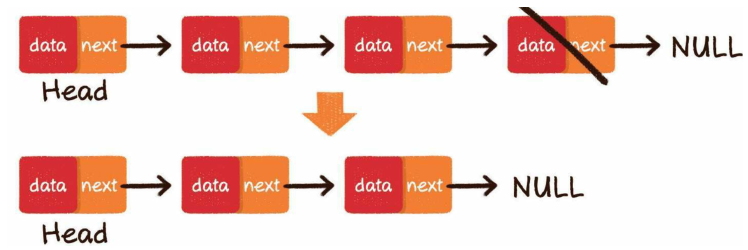
\includegraphics[scale=0.8]{img/C3/3-2/1.png}
\end{figure}

\subsubsection{中间删除}

把要删除的结点的前置结点的next指针,指向要删除结点的下一个结点。

\begin{figure}[H]
	\centering
	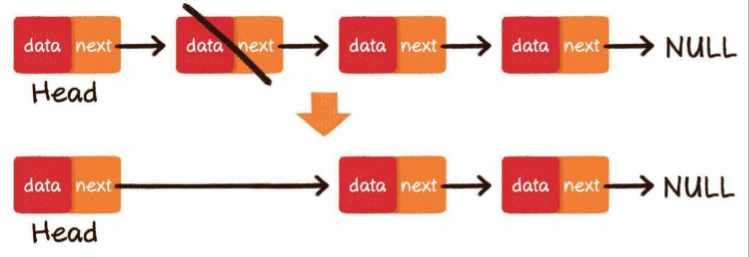
\includegraphics[scale=0.5]{img/C3/3-2/2.png}
\end{figure}

许多高级语言,如Java,拥有自动化的垃圾回收机制,所以不用刻意去释放被删除的结点,只要没有外部引用指向它们,被删除的结点会被自动回收。 \\

如果不考虑删除操作之前的查找的过程,只考虑纯粹的删除操作,时间复杂度是$ O(1) $。

\newpage

\section{带头结点的链表}

\subsection{带头结点的链表}

为了方便链表的插入、删除操作,在链表加上头结点之后,无论链表是否为空,头指针始终指向头结尾。因此对于空表和非空表的处理也统一了,方便了链表的操作,也减少了程序的复杂性和出现bug的机会。 \\

\mybox{插入结点}

\begin{lstlisting}[language=C]
void insert(List *head, int pos, dataType val) {
    Node *newNode = (Node *)malloc(sizeof(Node));
    newNode->data = val;
    newNode->next =  NULL;
    
    // 找到插入位置
    Node *temp = head;
    for(int i = 0; i < pos; i++) {
        temp = temp->next;
    }
    newNode->next = temp->next;
    temp->next = newNode;
}
\end{lstlisting}

\vspace{0.5cm}

\mybox{删除结点}

\begin{lstlisting}[language=C]
void delete(List *head, int pos) {
    Node *temp = head;
    for(int i = 0; i < pos; i++) {
        temp = temp->next;
    }
    Node *del = temp->next;
    temp->next = del->next;
    free(del);
    del = NULL;
}
\end{lstlisting}

\subsection{数组VS链表}

数据结构没有绝对的好与坏,数组和链表各有千秋。

\begin{table}[H]
	\centering
	\setlength{\tabcolsep}{5mm}{
		\begin{tabular}{|c|l|l|}
			\hline
			\textbf{比较内容} & \textbf{数组}          & \textbf{链表}                \\
			\hline
			基本              & 一组固定数量的数据项   & 可变数量的数据项             \\
			\hline
			大小              & 声明期间指定           & 无需指定,执行期间增长或收缩 \\
			\hline
			存储分配          & 元素位置在编译期间分配 & 元素位置在运行时分配         \\
			\hline
			元素顺序          & 连续存储               & 随机存储                     \\
			\hline
			访问元素          & 直接访问:索引、下标   & 顺序访问:指针遍历           \\
			\hline
			插入/删除         & 速度慢                 & 快速、高效                   \\
			\hline
			查找              & 线性查找、二分查找     & 线性查找                     \\
			\hline
			内存利用率        & 低效                   & 高效                         \\
			\hline
		\end{tabular}
	}
	\caption{数组VS链表}
\end{table}

数组的优势在于能够快速定位元素,对于读操作多、写操作少的场景来说,用数组更合适一些。 \\

相反,链表的优势在于能够灵活地进行插入和删除操作,如果需要频繁地插入、删除元素,用链表更合适一些。
% \chapter{栈}

\section{栈}

\subsection{栈(Stack)}

栈,又名堆栈,是一种运算受限的线性数据结构,栈只能在表尾进行插入和删除操作。 \\

栈中的元素只能先进后出(FILO, First In Last Out)。最早进入栈的元素所存放的位置叫作栈底(bottom),最后进入栈的元素存放的位置叫作栈顶(top)。 \\

\begin{figure}[H]
    \centering
    \begin{tikzpicture}
        \matrix[queue] (Q1) {
        |[fill=none, draw=none]| \\
        |(front)| C\\
        B\\
        |(rear)| A\\};
        \draw[green,thick,-] (Q1.north west) |-(Q1.south)-| (Q1.north east);
        \draw[<-] ([xshift=.2cm]front.east) -- ++ (0:.5) node[right] {top};
        \draw[<-] ([xshift=.2cm]rear.east) -- ++ (0:.5) node[right] {bottom};
        \draw[<-,very thick] (Q1.north) to[out=90,in=190] ++ (1,1) node[right, queue element] (D) {D};
        \node[below=3mm of Q1.south east] {before};

        \scope[xshift=3.5cm]
        \matrix[queue] (Q1) {
            |(front)| D \\
            C           \\
            B           \\
            |(rear)| A\\};
        \draw[green,thick,-] (Q1.north west) |-(Q1.south)-| (Q1.north east);
        \draw[<-] ([xshift=.2cm]front.east) -- ++ (0:.5) node[right] {top};
        \draw[<-] ([xshift=.2cm]rear.east) -- ++ (0:.5) node[right] {bottom};
        \node[below=3mm of Q1.south east] {after};
        \endscope
    \end{tikzpicture}
    \caption{栈}
\end{figure}

栈这种数据结构既可以用数组来实现,也可以用链表来实现。

\subsection{顺序栈}

使用数组方式实现的栈称为静态栈。可以根据下标来表示栈顶在数组中的位置,对于空栈,栈顶为-1。 \\

进行入栈操作时,栈顶指针+1;出栈时,栈顶指针-1。 \\

\begin{figure}[H]
    \centering
    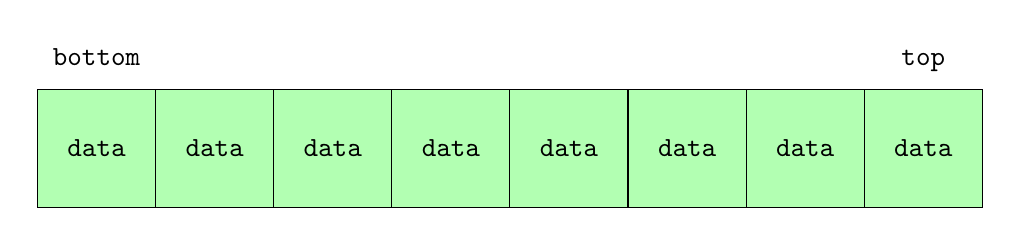
\begin{tikzpicture}[font=\ttfamily,
            array/.style={matrix of nodes,nodes={draw, minimum size=15mm, fill=green!30},column sep=-\pgflinewidth, row sep=0.5mm, nodes in empty cells,
                    row 1/.style={nodes={draw=none, fill=none, minimum size=5mm}},
                }]

        \matrix[array] (array) {
            bottom &      &      &      &      &      &      & top  \\
            data   & data & data & data & data & data & data & data \\
        };
    \end{tikzpicture}
    \caption{顺序栈}
\end{figure}

对满栈进行入栈和对空栈进行出栈操作操作都会产生数组的越界并引起程序崩溃,称为上溢和下溢。因此使用顺序栈前需要提前声明一个数组的大小,如果数组大小不够则可能发生数组越界,如果数组太大则会浪费一定的空间。 \\

使用数组实现的栈的执行效率会比用链表来实现的高,入栈和出栈不需要移动大量元素,只需要移动栈顶指针即可。 \\

\subsection{链式栈}

使用链表方式实现的栈称为动态栈。通过在表头插入一个元素来实现入栈,通过删除表尾元素来实现出栈。 \\

\begin{figure}[H]
    \centering
    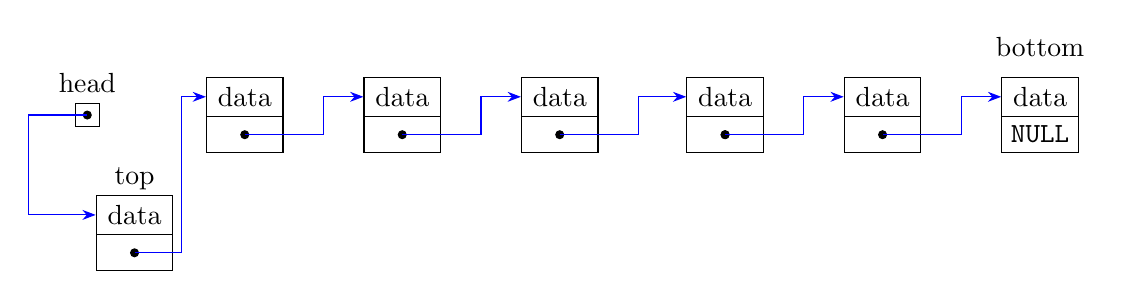
\begin{tikzpicture}[node distance=2cm, auto, scale=1,
            every node/.style={scale=1}]
        \node[head, label=above:head, xshift=-0.5cm] (head) {};
        \node[data, right of=head] (A) {\data};
        \node[above of=A,node distance=0.5cm] (a1){};
        \node[data, right of=A] (B) {\data};
        \node[above of=B,node distance=0.5cm] (a2){};
        \node[data, right of=B] (C) {\data};
        \node[above of=C,node distance=0.5cm] (a3){};
        \node[data, below of=head, xshift=0.6cm, yshift=0.5cm] (NEW) {\data};
        \node[above of=NEW,node distance=0.3cm,label=above:top] (new){};
        \node[data, right of=C, xshift=0.1cm] (D) {\data};%, xshift=1.5cm
        \node[above of=D,node distance=0.5cm] (a4){};
        \node[data, right of=D] (E) {\data};
        \node[above of=E,node distance=0.5cm] (a5){};
        \node[data, right of=E] (last) {data \nodepart{second} \texttt{NULL}};
        \node[above of=last,node distance=0.5cm,label=above:bottom] (a6){};

        \draw[fill] (head.center) circle (0.05);

        \path[ptr] (head.center) --++(left:7.5mm) |- (NEW.text west);
        \draw[fill] ($(NEW.south)!0.5!(NEW.text split)$) circle (0.05);
        \draw[ptr] ($(NEW.south)!0.5!(NEW.text split)$) --++(right:6mm) |- (A.text west);
        \draw[fill] ($(A.south)!0.5!(A.text split)$) circle (0.05);
        \draw[ptr] ($(A.south)!0.5!(A.text split)$) --++(right:10mm) |- (B.text west);
        \draw[fill] ($(B.south)!0.5!(B.text split)$) circle (0.05);
        \draw[ptr] ($(B.south)!0.5!(B.text split)$) --++(right:10mm) |- (C.text west);
        \draw[fill] ($(C.south)!0.5!(C.text split)$) circle (0.05);
        \draw[ptr] ($(C.south)!0.5!(C.text split)$) --++(right:10mm) |- (D.text west);
        \draw[fill] ($(D.south)!0.5!(D.text split)$) circle (0.05);
        \draw[fill] ($(D.south)!0.5!(D.text split)$) circle (0.05);
        \draw[ptr] ($(D.south)!0.5!(D.text split)$) --++(right:10mm) |- (E.text west);
        \draw[fill] ($(E.south)!0.5!(E.text split)$) circle (0.05);
        \draw[ptr] ($(E.south)!0.5!(E.text split)$) --++(right:10mm) |- (last.text west);
    \end{tikzpicture}
    \caption{链式栈}
\end{figure}

动态栈有链表的部分特性,元素与元素之间在物理存储上可以不连续,但是功能有些受限制,动态栈只能在栈顶处进行插入和删除操作,不能在栈尾或栈中间进行插入和删除操作。 \\

动态栈的元素内存是动态分配的,避免了静态栈可能会浪费空间的问题,但是对申请和释放空间的调用开销会比较大。

\subsection{栈的应用}

栈的输出顺序和输入顺序相反,所以栈同行用于对历史的回溯。例如实现递归的逻辑,就可以用栈回溯调用链。 \\

\begin{figure}[H]
    \centering
    \begin{drawstack}
        \startframe
        \cell{N = 1}
        \cell{...}
        \finishframe{fact(1)}
        \startframe
        \cell{N = 2}
        \cell{...}
        \finishframe{fact(2)}
        \cell{$ \vdots $}
        \startframe
        \cell{N = 5}
        \cell{...}
        \finishframe{fact(5)}
    \end{drawstack}
    \caption{函数调用栈}
\end{figure}

栈还有一个著名的应用场景就是面包屑导航,使用户在流浪页面时可以轻松地回溯到上一级更更上一级页面。

\begin{figure}[H]
    \centering
    
\includegraphics[]{img/C4/4-1/1.png}
    \caption{面包屑导航}
\end{figure}

\newpage

\section{入栈与出栈}

\subsection{入栈(Push)}

入栈操作就是把新元素放入栈中,只允许从栈顶一侧放入元素,新元素的位置将会成为新的栈顶。最初,栈为空,栈顶的初始值为-1。每当向栈中添加元素时,栈顶指针+1。 \\

入栈只影响最后一个元素,不涉及元素的整体移动,所以无论是以数组还是链表实现,时间复杂度都是$ O(1) $。 \\

\mybox{入栈}

\begin{lstlisting}[language=C]
void push(Stack *stack, dataType val) {
    stack->data[++stack->top] = val;
}
\end{lstlisting}

\subsection{出栈(Pop)}

出栈操作就是把新元素从栈中弹出,只有栈顶元素才允许出栈,出栈元素的前一个元素将会成为新的栈顶。从栈中移出元素,栈顶指针-1。数组中元素的删除并非真正意义上把元素从内存中清除,出栈只需对栈顶-1即可,后期向栈中添加元素时,新元素会将旧元素覆盖。 \\

出栈只影响最后一个元素,不涉及元素的整体移动,所以无论是以数组还是链表实现,时间复杂度都是$ O(1) $。 \\

\mybox{出栈}

\begin{lstlisting}[language=C]
dataType pop(Stack *stack) {
    return stack->data[stack->top--];
}
\end{lstlisting}

\newpage

\section{最小栈}

\subsection{最小栈}

设计一个支持push()、pop()、peek()和getMin()操作的栈,并能在常数时间内检索到最小元素。 \\

对于栈来说,如果一个元素a在入栈时,栈里有其它的元素b、c、d,那么无论这个栈在之后经历了什么操作,只要a在栈中,b、c、d就一定在栈中。因此,在操作过程中的任意一个时刻,只要栈顶的元素是a,那么就可以确定栈里面现在的元素一定是a、b、c、d。 \\

那么可以在每个元素a入栈时把当前栈的最小值m存储起来。在这之后无论何时,如果栈顶元素是a,就可以直接返回存储的最小值m。 \\

当一个元素要入栈时,取辅助栈的栈顶存储的最小值,与当前元素比较得出最小值,将这个最小值插入辅助栈中。当一个元素要出栈时,把辅助栈的栈顶元素也一并弹出。这样在任意一个时刻,栈内元素的最小值就存储在辅助栈的栈顶元素中。 \\

\mybox{最小栈}

\begin{lstlisting}[language=Python]
class MinStack:
    def __init__(self):
        self.stack = []
        self.min_stack = [math.inf]
    
    def push(self, data):
        self.stack.append(data)
        self.min_stack.append(min(data, self.min_stack[-1]))
    
    def pop(self):
        self.stack.pop()
        self.min_stack.pop()
    
    def peek(self):
        return self.stack[-1]
    
    def get_min(self):
        return self.min_stack[-1]
\end{lstlisting}

\newpage

\section{括号匹配}

\subsection{括号匹配}

给定一个只包括"("、")"、"["、"]"、"\{"和"\}"的字符串,判断字符串是否有效。有效字符串需满足左括号必须用相同类型的右括号闭合,并且左括号必须以正确的顺序闭合。 \\

判断括号的有效性可以使用栈来解决。通过遍历字符串,当遇到左括号时,会期望在后续的遍历中,有一个相同类型的右括号将其闭合。由于后遇到的左括号要先闭合,因此将这个左括号放入栈顶。 \\

当遇到右括号时,需要将一个相同类型的左括号闭合。此时可以取出栈顶的左括号并判断它们是否是相同类型的括号。如果不是相同的类型,或者栈中并没有左括号,那么字符串无效。在遍历结束后,如果为空栈,说明字符串中的所有左括号闭合。 \\

注意有效字符串的长度一定为偶数,因此如果字符串的长度为奇数,可以直接返回判断出字符串无效,省去后续的遍历判断过程。 \\

\mybox{括号匹配}

\begin{lstlisting}[language=Python]
def valid_paratheses(s):
    if len(s) % 2 == 1:
        return False
    
    pairs = {")": "(", "]": "[", "}": "{"}
    stack = list()
    for paran in s:
        if paran in pairs:
            if not stack or stack[-1] != pairs[paran]:
                return False
            stack.pop()
        else:
            stack.append(paran)

    return not stack
\end{lstlisting}

\newpage

\section{表达式求值}

\subsection{表达式求值}

逆波兰表达式是一种后缀表达式,所谓后缀就是指运算符写在运算数的后面。平常使用的算式则是一种中缀表达式,如$ (1 + 2) * (3 + 4) $,该算式的逆波兰表达式写法为$ 1\ 2 + 3\ 4 + * $。 \\

逆波兰表达式的优点在于去掉了中缀表达式中的括号后表达式无歧义,因此适合用栈操作运算。遇到数字则入栈,遇到算符则取出栈顶两个数字进行计算,并将结果压入栈中。 \\

在对中缀表达式求值时,一般都会将其转换为后缀表达式的形式,转换过程同样需要用到栈,规则如下:

\begin{enumerate}
    \item 如果遇到操作数,就直接将其输出。

    \item 如果遇到左括号,将其放入栈中。

    \item 如果遇到右括号,则一直出栈并输出,直到遇到左括号为止。注意,左括号只出栈并不输出。

    \item 如果遇到任何其它的运算符,如果为栈为空,则直接入栈。否则从栈中出栈元素并输出,直到遇到优先级更低的元素(或者栈为空)位置。在出栈完这些元素后,再将当前遇到的运算符入栈。有一点需要注意,只有在遇到右括号的情况下才将左括号出栈,其它情况都不会出栈左括号。

    \item 如果读取到了表达式的末尾,则将栈中所有元素依次出栈输出。
\end{enumerate}

\begin{figure}[H]
    \centering
    \begin{tikzpicture}[]
        \draw[-] (0,0) rectangle (7,1);
        \draw[-] (1,0) -- (1,1);
        \draw[-] (2,0) -- (2,1);
        \draw[-] (3,0) -- (3,1);
        \draw[-] (4,0) -- (4,1);
        \draw[-] (5,0) -- (5,1);
        \draw[-] (6,0) -- (6,1);
        \draw[-] (7,0) -- (7,1);

        \draw (0.5,0.5) node{1};
        \draw (1.5,0.5) node{*};
        \draw (2.5,0.5) node{(};
        \draw (3.5,0.5) node{2};
        \draw (4.5,0.5) node{+};
        \draw (5.5,0.5) node{3};
        \draw (6.5,0.5) node{)};

        \draw[-] (8,3) rectangle (9,-2);
        \draw[-] (8,2) -- (9,2);
        \draw[-] (8,1) -- (9,1);
        \draw[-] (8,0) -- (9,0);
        \draw[-] (8,-1) -- (9,-1);
        \draw (8.5,-2.5) node{num};

        \draw[-] (10,3) rectangle (11,-2);
        \draw[-] (10,2) -- (11,2);
        \draw[-] (10,1) -- (11,1);
        \draw[-] (10,0) -- (11,0);
        \draw[-] (10,-1) -- (11,-1);
        \draw (10.5,-2.5) node{op};

        \draw (8.5,-1.5) node{1};
        \draw[->, red] (0.5,0) to[bend right] (8,-1.5);
    \end{tikzpicture}
\end{figure}

\begin{figure}[H]
    \centering
    \begin{tikzpicture}[]
        \draw[-] (0,0) rectangle (7,1);
        \draw[-] (1,0) -- (1,1);
        \draw[-] (2,0) -- (2,1);
        \draw[-] (3,0) -- (3,1);
        \draw[-] (4,0) -- (4,1);
        \draw[-] (5,0) -- (5,1);
        \draw[-] (6,0) -- (6,1);
        \draw[-] (7,0) -- (7,1);

        \draw (0.5,0.5) node{1};
        \draw (1.5,0.5) node{*};
        \draw (2.5,0.5) node{(};
        \draw (3.5,0.5) node{2};
        \draw (4.5,0.5) node{+};
        \draw (5.5,0.5) node{3};
        \draw (6.5,0.5) node{)};

        \draw[-] (8,3) rectangle (9,-2);
        \draw[-] (8,2) -- (9,2);
        \draw[-] (8,1) -- (9,1);
        \draw[-] (8,0) -- (9,0);
        \draw[-] (8,-1) -- (9,-1);
        \draw (8.5,-2.5) node{num};

        \draw[-] (10,3) rectangle (11,-2);
        \draw[-] (10,2) -- (11,2);
        \draw[-] (10,1) -- (11,1);
        \draw[-] (10,0) -- (11,0);
        \draw[-] (10,-1) -- (11,-1);
        \draw (10.5,-2.5) node{op};

        \draw (8.5,-1.5) node{1};
        \draw (10.5,-1.5) node{*};
        \draw[->, red] (1.5,0) to[bend right] (10,-1.5);
    \end{tikzpicture}
\end{figure}

\begin{figure}[H]
    \centering
    \begin{tikzpicture}[]
        \draw[-] (0,0) rectangle (7,1);
        \draw[-] (1,0) -- (1,1);
        \draw[-] (2,0) -- (2,1);
        \draw[-] (3,0) -- (3,1);
        \draw[-] (4,0) -- (4,1);
        \draw[-] (5,0) -- (5,1);
        \draw[-] (6,0) -- (6,1);
        \draw[-] (7,0) -- (7,1);

        \draw (0.5,0.5) node{1};
        \draw (1.5,0.5) node{*};
        \draw (2.5,0.5) node{(};
        \draw (3.5,0.5) node{2};
        \draw (4.5,0.5) node{+};
        \draw (5.5,0.5) node{3};
        \draw (6.5,0.5) node{)};

        \draw[-] (8,3) rectangle (9,-2);
        \draw[-] (8,2) -- (9,2);
        \draw[-] (8,1) -- (9,1);
        \draw[-] (8,0) -- (9,0);
        \draw[-] (8,-1) -- (9,-1);
        \draw (8.5,-2.5) node{num};

        \draw[-] (10,3) rectangle (11,-2);
        \draw[-] (10,2) -- (11,2);
        \draw[-] (10,1) -- (11,1);
        \draw[-] (10,0) -- (11,0);
        \draw[-] (10,-1) -- (11,-1);
        \draw (10.5,-2.5) node{op};

        \draw (8.5,-1.5) node{1};
        \draw (10.5,-1.5) node{*};
        \draw (10.5,-0.5) node{(};
        \draw[->, red] (2.5,0) to[bend right] (10,-0.5);
    \end{tikzpicture}
\end{figure}

\begin{figure}[H]
    \centering
    \begin{tikzpicture}[]
        \draw[-] (0,0) rectangle (7,1);
        \draw[-] (1,0) -- (1,1);
        \draw[-] (2,0) -- (2,1);
        \draw[-] (3,0) -- (3,1);
        \draw[-] (4,0) -- (4,1);
        \draw[-] (5,0) -- (5,1);
        \draw[-] (6,0) -- (6,1);
        \draw[-] (7,0) -- (7,1);

        \draw (0.5,0.5) node{1};
        \draw (1.5,0.5) node{*};
        \draw (2.5,0.5) node{(};
        \draw (3.5,0.5) node{2};
        \draw (4.5,0.5) node{+};
        \draw (5.5,0.5) node{3};
        \draw (6.5,0.5) node{)};

        \draw[-] (8,3) rectangle (9,-2);
        \draw[-] (8,2) -- (9,2);
        \draw[-] (8,1) -- (9,1);
        \draw[-] (8,0) -- (9,0);
        \draw[-] (8,-1) -- (9,-1);
        \draw (8.5,-2.5) node{num};

        \draw[-] (10,3) rectangle (11,-2);
        \draw[-] (10,2) -- (11,2);
        \draw[-] (10,1) -- (11,1);
        \draw[-] (10,0) -- (11,0);
        \draw[-] (10,-1) -- (11,-1);
        \draw (10.5,-2.5) node{op};

        \draw (8.5,-1.5) node{1};
        \draw (10.5,-1.5) node{*};
        \draw (10.5,-0.5) node{(};
        \draw (8.5,-0.5) node{2};
        \draw[->, red] (3.5,0) to[bend right] (8,-0.5);
    \end{tikzpicture}
\end{figure}

\begin{figure}[H]
    \centering
    \begin{tikzpicture}[]
        \draw[-] (0,0) rectangle (7,1);
        \draw[-] (1,0) -- (1,1);
        \draw[-] (2,0) -- (2,1);
        \draw[-] (3,0) -- (3,1);
        \draw[-] (4,0) -- (4,1);
        \draw[-] (5,0) -- (5,1);
        \draw[-] (6,0) -- (6,1);
        \draw[-] (7,0) -- (7,1);

        \draw (0.5,0.5) node{1};
        \draw (1.5,0.5) node{*};
        \draw (2.5,0.5) node{(};
        \draw (3.5,0.5) node{2};
        \draw (4.5,0.5) node{+};
        \draw (5.5,0.5) node{3};
        \draw (6.5,0.5) node{)};

        \draw[-] (8,3) rectangle (9,-2);
        \draw[-] (8,2) -- (9,2);
        \draw[-] (8,1) -- (9,1);
        \draw[-] (8,0) -- (9,0);
        \draw[-] (8,-1) -- (9,-1);
        \draw (8.5,-2.5) node{num};

        \draw[-] (10,3) rectangle (11,-2);
        \draw[-] (10,2) -- (11,2);
        \draw[-] (10,1) -- (11,1);
        \draw[-] (10,0) -- (11,0);
        \draw[-] (10,-1) -- (11,-1);
        \draw (10.5,-2.5) node{op};

        \draw (8.5,-1.5) node{1};
        \draw (10.5,-1.5) node{*};
        \draw (10.5,-0.5) node{(};
        \draw (8.5,-0.5) node{2};
        \draw (10.5,0.5) node{+};
        \draw[->, red] (4.5,0) to[bend right] (10,0.5);
    \end{tikzpicture}
\end{figure}

\begin{figure}[H]
    \centering
    \begin{tikzpicture}[]
        \draw[-] (0,0) rectangle (7,1);
        \draw[-] (1,0) -- (1,1);
        \draw[-] (2,0) -- (2,1);
        \draw[-] (3,0) -- (3,1);
        \draw[-] (4,0) -- (4,1);
        \draw[-] (5,0) -- (5,1);
        \draw[-] (6,0) -- (6,1);
        \draw[-] (7,0) -- (7,1);

        \draw (0.5,0.5) node{1};
        \draw (1.5,0.5) node{*};
        \draw (2.5,0.5) node{(};
        \draw (3.5,0.5) node{2};
        \draw (4.5,0.5) node{+};
        \draw (5.5,0.5) node{3};
        \draw (6.5,0.5) node{)};

        \draw[-] (8,3) rectangle (9,-2);
        \draw[-] (8,2) -- (9,2);
        \draw[-] (8,1) -- (9,1);
        \draw[-] (8,0) -- (9,0);
        \draw[-] (8,-1) -- (9,-1);
        \draw (8.5,-2.5) node{num};

        \draw[-] (10,3) rectangle (11,-2);
        \draw[-] (10,2) -- (11,2);
        \draw[-] (10,1) -- (11,1);
        \draw[-] (10,0) -- (11,0);
        \draw[-] (10,-1) -- (11,-1);
        \draw (10.5,-2.5) node{op};

        \draw (8.5,-1.5) node{1};
        \draw (10.5,-1.5) node{*};
        \draw (10.5,-0.5) node{(};
        \draw (8.5,-0.5) node{2};
        \draw (10.5,0.5) node{+};
        \draw (8.5,0.5) node{3};
        \draw[->, red] (5.5,1) to[bend left] (8,0.5);
    \end{tikzpicture}
\end{figure}

\begin{figure}[H]
    \centering
    \begin{tikzpicture}[]
        \draw[-] (0,0) rectangle (7,1);
        \draw[-] (1,0) -- (1,1);
        \draw[-] (2,0) -- (2,1);
        \draw[-] (3,0) -- (3,1);
        \draw[-] (4,0) -- (4,1);
        \draw[-] (5,0) -- (5,1);
        \draw[-] (6,0) -- (6,1);
        \draw[-] (7,0) -- (7,1);

        \draw (0.5,0.5) node{1};
        \draw (1.5,0.5) node{*};
        \draw (2.5,0.5) node{(};
        \draw (3.5,0.5) node{2};
        \draw (4.5,0.5) node{+};
        \draw (5.5,0.5) node{3};
        \draw (6.5,0.5) node{)};

        \draw[-] (8,3) rectangle (9,-2);
        \draw[-] (8,2) -- (9,2);
        \draw[-] (8,1) -- (9,1);
        \draw[-] (8,0) -- (9,0);
        \draw[-] (8,-1) -- (9,-1);
        \draw (8.5,-2.5) node{num};

        \draw[-] (10,3) rectangle (11,-2);
        \draw[-] (10,2) -- (11,2);
        \draw[-] (10,1) -- (11,1);
        \draw[-] (10,0) -- (11,0);
        \draw[-] (10,-1) -- (11,-1);
        \draw (10.5,-2.5) node{op};

        \draw (8.5,-1.5) node{1};
        \draw (10.5,-1.5) node{*};
        \draw (10.5,-0.5) node{(};
        \draw (8.5,-0.5) node{2};
        \draw (10.5,0.5) node{+};
        \draw (8.5,0.5) node{3};
        \draw[->, red] (6.5,2) -- (6.5,1);
        \draw[->, red] (10,0.5) -- (9,1.5);
        \draw[->, red] (11,-0.5) -- (12,-0.5);
    \end{tikzpicture}
\end{figure}

\begin{figure}[H]
    \centering
    \begin{tikzpicture}[]
        \draw[-] (0,0) rectangle (7,1);
        \draw[-] (1,0) -- (1,1);
        \draw[-] (2,0) -- (2,1);
        \draw[-] (3,0) -- (3,1);
        \draw[-] (4,0) -- (4,1);
        \draw[-] (5,0) -- (5,1);
        \draw[-] (6,0) -- (6,1);
        \draw[-] (7,0) -- (7,1);

        \draw (0.5,0.5) node{1};
        \draw (1.5,0.5) node{*};
        \draw (2.5,0.5) node{(};
        \draw (3.5,0.5) node{2};
        \draw (4.5,0.5) node{+};
        \draw (5.5,0.5) node{3};
        \draw (6.5,0.5) node{)};

        \draw[-] (8,3) rectangle (9,-2);
        \draw[-] (8,2) -- (9,2);
        \draw[-] (8,1) -- (9,1);
        \draw[-] (8,0) -- (9,0);
        \draw[-] (8,-1) -- (9,-1);
        \draw (8.5,-2.5) node{num};

        \draw[-] (10,3) rectangle (11,-2);
        \draw[-] (10,2) -- (11,2);
        \draw[-] (10,1) -- (11,1);
        \draw[-] (10,0) -- (11,0);
        \draw[-] (10,-1) -- (11,-1);
        \draw (10.5,-2.5) node{op};

        \draw (8.5,-1.5) node{1};
        \draw (10.5,-1.5) node{*};
        \draw (8.5,-0.5) node{2};
        \draw (8.5,0.5) node{3};
        \draw (8.5,1.5) node{+};
        \draw[->, red] (10,-1.5) -- (9,2.5);
    \end{tikzpicture}
\end{figure}

\begin{figure}[H]
    \centering
    \begin{tikzpicture}[]
        \draw[-] (0,0) rectangle (7,1);
        \draw[-] (1,0) -- (1,1);
        \draw[-] (2,0) -- (2,1);
        \draw[-] (3,0) -- (3,1);
        \draw[-] (4,0) -- (4,1);
        \draw[-] (5,0) -- (5,1);
        \draw[-] (6,0) -- (6,1);
        \draw[-] (7,0) -- (7,1);

        \draw (0.5,0.5) node{1};
        \draw (1.5,0.5) node{*};
        \draw (2.5,0.5) node{(};
        \draw (3.5,0.5) node{2};
        \draw (4.5,0.5) node{+};
        \draw (5.5,0.5) node{3};
        \draw (6.5,0.5) node{)};

        \draw[-] (8,3) rectangle (9,-2);
        \draw[-] (8,2) -- (9,2);
        \draw[-] (8,1) -- (9,1);
        \draw[-] (8,0) -- (9,0);
        \draw[-] (8,-1) -- (9,-1);
        \draw (8.5,-2.5) node{num};

        \draw[-] (10,3) rectangle (11,-2);
        \draw[-] (10,2) -- (11,2);
        \draw[-] (10,1) -- (11,1);
        \draw[-] (10,0) -- (11,0);
        \draw[-] (10,-1) -- (11,-1);
        \draw (10.5,-2.5) node{op};

        \draw (8.5,-1.5) node{1};
        \draw (8.5,-0.5) node{2};
        \draw (8.5,0.5) node{3};
        \draw (8.5,1.5) node{+};
        \draw (8.5,2.5) node{*};
    \end{tikzpicture}
\end{figure}

\mybox{表达式求值}

\begin{lstlisting}[language=Python]
def priority(op):
    """
        运算符的优先级
        乘除法优先级高于加减法
        Args:
            op (str): 运算符
        Returns:
            (int): 优先级
    """
    if op == "*" or op == "/":
        return 2
    elif op == "+" or op == "-":
        return 1
    else:
        return 0

def infix_to_postfix(exp):
    """
        中缀表达式转换后缀表达式
        转换后的后缀表达式操作数之前带空格
        Args:
            exp (str): 中缀表达式
        Returns:
            (str): 后缀表达式
    """
    postfix = ""    # 保存生成的后缀表达式
    s = stack.Stack()

    number = ""
    for ch in exp:
        # 如果是数字,保存每一位数字
        if ch.isdigit():
            number += ch
            continue
        
        # 如果读取一个完整数字,直接输出
        if len(number) > 0:
            postfix += number + " "
            number = ""
        
        # 空格忽略
        if ch == " ":
            continue
        
        # 如果是运算符,并且空栈,则直接入栈
        if s.is_empty():
            s.push(ch)
        # 如果遇到左括号,将其放入栈中
        elif ch == "(":
            s.push(ch)
        # 如果遇到右括号,则一直出栈并输出,直到遇到左括号为止
        # 注意,左括号只出栈并不输出
        elif ch == ")":
            while s.peek() != "(":
                postfix += s.pop() + " "
            s.pop()
        # 如果遇到任何其它的运算符,如果为栈为空,则直接入栈
        # 否则从栈中出栈元素并输出,直到遇到优先级更低的元素(或为空)
        # 在出栈完这些元素后,再将当前遇到的运算符入栈
        # 只有遇到右括号的情况下才将左括号出栈
        else:
            while not s.is_empty() 
                    and priority(ch) <= priority(s.peek()):
                postfix += s.pop() + " "
            s.push(ch)
    
    # 如果读取一个完整数字,直接输出
    if len(number) > 0:
        postfix += number + " "
        number = ""
    
    while not s.is_empty():
        postfix += s.pop() + " "
    
    return postfix.rstrip()

def calculate(postfix):
    """
    表达式求值
    Args:
        postfix (str): 后缀表达式
    Returns:
        (int): 表达式结果
    """
    s = stack.Stack()

    tokens = postfix.split()
    for token in tokens:
        # 数字则入栈
        try:
            s.push(int(token))
        # 运算符则出栈2次,将计算结果入栈
        except ValueError:
            num2 = s.pop()
            num1 = s.pop()
            if token == '+':
                s.push(num1 + num2)
            elif token == '-':
                s.push(num1 - num2)
            elif token == '*':
                s.push(num1 * num2)
            elif token == '/':
                s.push(int(num1 / num2))
    return s.pop()
\end{lstlisting}

\newpage
% \chapter{队列}

\section{队列}

\subsection{队列(Queue)}

队列是一种运算受限的线性数据结构,不同于栈的先进后出(FILO),队列中的元素只能先进先出(FIFO, First In First Out)。 \\

队列的出口端叫作队头(front),队列的入口端叫作队尾(rear)。队列只允许在队尾进行入队(enqueue),在队头进行出队(dequeue)。 \\

与栈类似,队列既可以用数组来实现,也可以用链表来实现。其中用数组实现时,为了入队操作的方便,把队尾位置规定为最后入队元素的下一个位置。 \\


\chapter{哈希表}

\section{哈希表}

\subsection{哈希表(Hash Table)}

例如开发一个学生管理系统,需要有通过输入学号快速查出对应学生的姓名的功能。这里不必每次都去查询数据库,而可以在内存中建立一个缓存表,这样做可以提高查询效率。

\begin{table}[H]
	\centering
	\setlength{\tabcolsep}{5mm}{
		\begin{tabular}{|c|c|}
			\hline
			\textbf{学号} & \textbf{姓名} \\
			\hline
			001121        & 张三          \\
			\hline
			002123        & 李四          \\
			\hline
			002931        & 王五          \\
			\hline
			003278        & 赵六          \\
			\hline
		\end{tabular}
	}
	\caption{学生名单}
\end{table}

再例如需要统计一本英文书里某些单词出现的频率,就需要遍历整本书的内容,把这些单词出现的次数记录在内存中。

\begin{table}[H]
	\centering
	\setlength{\tabcolsep}{5mm}{
		\begin{tabular}{|c|c|}
			\hline
			\textbf{单词} & \textbf{出现次数} \\
			\hline
			this          & 108               \\
			\hline
			and           & 56                \\
			\hline
			are           & 79                \\
			\hline
			by            & 46                \\
			\hline
		\end{tabular}
	}
	\caption{词频统计}
\end{table}

因为这些需要,一个重要的数据结构诞生了,这个数据结构就是哈希表。哈希表也称散列表,哈希表提供了键(key)和值(value)的映射关系,只要给出一个key,就可以高效地查找到它所匹配的value。 \\

哈希表的时间复杂度几乎是常量$ O(1) $,即查找时间与问题规模无关。 \\

哈希表的两项基本工作:

\begin{enumerate}
	\item 计算位置:构造哈希函数确定关键字的存储位置。
	\item 解决冲突:应用某种策略解决多个关键字位置相同的问题。
\end{enumerate}

\newpage

\section{哈希函数}

\subsection{哈希函数(Hash Function)}

哈希的基本思想是将键key通过一个确定的函数,计算出对应的函数值value作为数据对象的存储地址,这个函数就是哈希函数。

\begin{figure}[H]
	\centering
	\begin{tikzpicture}
		\draw (0,0.5) circle (1) node{h(key)};

		\draw (-4,5) node{key};
		\draw[-] (-5,4) rectangle (-3,3);
		\draw[-] (-5,2) rectangle (-3,1);
		\draw[-] (-5,0) rectangle (-3,-1);
		\draw[-] (-5,-2) rectangle (-3,-3);

		\draw (-4,3.5) node{张三};
		\draw (-4,1.5) node{李四};
		\draw (-4,-0.5) node{王五};
		\draw (-4,-2.5) node{赵六};

		\draw (4,5) node{hash table};
		\draw (3,4) rectangle (5,-3);
		\draw (3,3) -- (5,3);
		\draw (3,2) -- (5,2);
		\draw (3,1) -- (5,1);
		\draw (3,0) -- (5,0);
		\draw (3,-1) -- (5,-1);
		\draw (3,-2) -- (5,-2);

		\draw (4,-0.5) node{张三};
		\draw (4,3.5) node{李四};
		\draw (4,0.5) node{王五};
		\draw (4,-2.5) node{赵六};

		\draw[dashed, ->] (-3,3.5) -- (-1,0.5);
		\draw[dashed, ->] (-3,1.5) -- (-1,0.5);
		\draw[dashed, ->] (-3,-0.5) -- (-1,0.5);
		\draw[dashed, ->] (-3,-2.5) -- (-1,0.5);

		\draw[dashed, ->] (1,0.5) -- (3,-0.5);
		\draw[dashed, ->] (1,0.5) -- (3,3.5);
		\draw[dashed, ->] (1,0.5) -- (3,0.5);
		\draw[dashed, ->] (1,0.5) -- (3,-2.5);
	\end{tikzpicture}
	\caption{哈希函数}
\end{figure}

哈希表本质上也是一个数组,可是数组只能根据下标来访问,而哈希表的key则是以字符串类型为主的。 \\

在不同的语言中,哈希函数的实现方式是不一样的。假设需要存储整型变量,转化为数组的下标就不难实现了。最简单的转化方式就是按照数组长度进行取模运算。 \\

一个好的哈希函数应该考虑两个因素:

\begin{enumerate}
	\item 计算简单,以便提高转换速度。
	\item 关键字对应的地址空间分布均匀,以尽量减少冲突。
\end{enumerate}

\subsection{数字关键字的哈希函数构造方法}

对于数字类型的关键字,哈希函数有以下几种常用的构造方法:

\subsubsection{直接定址法}

取关键字的某个线性函数值为散列地址。

\vspace{-0.5cm}

$$
	h(key) = a * key + b
$$

例如根据出生年份计算人口数量h(key) = key - 1990:

\begin{table}[H]
	\centering
	\setlength{\tabcolsep}{5mm}{
		\begin{tabular}{|c|c|c|}
			\hline
			\textbf{地址} & \textbf{出生年份} & \textbf{人数} \\
			\hline
			0             & 1990              & 1285万        \\
			\hline
			1             & 1991              & 1281万        \\
			\hline
			2             & 1992              & 1280万        \\
			\hline
			$ \dots $     & $ \dots $         & $ \dots $     \\
			\hline
			10            & 2000              & 1250万        \\
			\hline
			$ \dots $     & $ \dots $         & $ \dots $     \\
			\hline
			21            & 2011              & 1180万        \\
			\hline
		\end{tabular}
	}
	\caption{直接定址法}
\end{table}

\subsubsection{除留余数法}

哈希函数为h(key) = key \% p,p一般取素数。 \\

例如h(key) = key \% 17:

\begin{table}[H]
	\centering
	\setlength{\tabcolsep}{1.5mm}{
		\begin{tabular}{|c|c|c|c|c|c|c|c|c|c|c|c|c|c|c|c|c|c|}
			\hline
			\textbf{地址}   & \textbf{0} & \textbf{1} & \textbf{2} & \textbf{3} & \textbf{4} & \textbf{5} & \textbf{6} & \textbf{7} & \textbf{8} & \textbf{9} & \textbf{10} & \textbf{11} & \textbf{12} & \textbf{13} & \textbf{14} & \textbf{15} & \textbf{16} \\
			\hline
			\textbf{关键字} & 34         & 18         & 2          & 20         &            &            & 23         & 7          & 42         &            & 27          & 11          &             & 30          &             & 15          &             \\
			\hline
		\end{tabular}
	}
	\caption{除留余数法}
\end{table}

\subsubsection{数字分析法}

分析数字关键字在各位上的变化情况,取比较随机的位作为散列地址。 \\

例如取11位手机号码的后4位作为地址h(key) = int(key + 7)。 \\

再例如取18位身份证号码中变化较为随机的位数:

\begin{table}[H]
	\centering
	\begin{tabular}{|c|c|c|c|c|c|c|c|c|c|c|c|c|c|c|c|c|c|c|}
		\hline
		\textbf{1}               & \textbf{2}               & \textbf{3}               & \textbf{4}               & \textbf{5}               & \textbf{6}               & \textbf{7}               & \textbf{8} & \textbf{9} & \textbf{10} & \textbf{11} & \textbf{12} & \textbf{13} & \textbf{14} & \textbf{15} & \textbf{16} & \textbf{17} & \textbf{18} \\
		\hline
		3                        & 3                        & 0                        & 1                        & 0                        & 6                        & 1                        & 9          & 9          & 0           & 1           & 0           & 0           & 8           & 0           & 4           & 1           & 9           \\
		\hline
		\multicolumn{2}{|c|}{省} & \multicolumn{2}{|c|}{市} & \multicolumn{2}{|c|}{区} & \multicolumn{4}{|c|}{年} & \multicolumn{2}{|c|}{月} & \multicolumn{2}{|c|}{日} & \multicolumn{3}{|c|}{辖} & 校验                                                                                                                                                  \\
		\hline
	\end{tabular}
	\caption{数字分析法}
\end{table}

\subsubsection{折叠法}

把关键字分割成位数相同的几个部分,然后叠加。 \\

例如将整数56793542每三位进行分割:

\begin{table}[H]
	\centering
	\begin{tabular}{cD{.}{.}{3}}
		  & 542  \\
		  & 793  \\
		+ & 056  \\
		\hline
		= & 1319
	\end{tabular}
\end{table}

\vspace{-1cm}

$$
	h(56793542) = 319
$$

\subsubsection{平方取中法}

计算关键字的平方,取中间几位。 \\

例如整数56793542:

\begin{table}[H]
	\centering
	\begin{tabular}{cD{.}{.}{3}}
		  & 56793542         \\
		* & 56793542         \\
		\hline
		= & 3225506412905764
	\end{tabular}
\end{table}

\vspace{-1cm}

$$
	h(56793542) = 641
$$

\subsection{字符串关键字的哈希函数构造方法}

对于字符串类型的关键字,哈希函数有以下几种常用的构造方法:

\subsubsection{ASCII码加和法}

\vspace{-0.5cm}

$$
	h(key) = \left(\sum key[i] \right)\ mod\ N
$$

但是对于某些字符串会导致严重冲突,例如:a3、b2、c1或eat、tea等。 \\

\subsubsection{移位法}

取前3个字符移位。

\vspace{-0.5cm}

$$
	h(key) = \left(key[0] \times 27^2 + key[1] \times 27 | key[2] \right)\ mod\ N
$$

对于一些字符串仍然会冲突,例如string、strong、street、structure等。 \\

一个有效的改进是涉及关键字中所有n个字符:

$$
	h(key) = \left( \sum_{i=0}^{n-1} key[n-i-1] \times 32^i \right)\ mod\ N
$$

\mybox{哈希函数} \\

快速计算$ h('abcde') = a * 32^4 + b * 32^3 + c * 32^2 + d * 32 + e $

\begin{lstlisting}[language=C]
int hash(char *key, int tableSize) {
    int h = 0;          // hash value
    int i = 0;
    while(key[i] != '\0') {
        h = (h << 5) + key[i];
        i++;
    }
    return h % tableSize;
}
\end{lstlisting}

\vspace{0.5cm}

\mybox{凯撒加密}

\begin{lstlisting}[language=C]
/**
* @brief  凯撒加密
* @note  加密算法:ciphertext[i] = (plaintext[i] + Key) % 128
* @param  plaintext: 明文
* @retval 密文
*/
char* encrypt(char *plaintext) {
    int n = strlen(plaintext);
    char *ciphertext = (char *)malloc((n + 1) * sizeof(char));
    for(int i = 0; i < n; i++) {
        ciphertext[i] = (plaintext[i] + KEY) % 128;
    }
    ciphertext[n] = '\0';
    return ciphertext;
}

/**
* @brief  凯撒解密
* @note   解密算法:plaintext[i] = (ciphertext[i] - key + 128) % 128
* @param  ciphertext: 密文
* @retval 明文
*/
char* decrypt(char *ciphertext) {
    int n = strlen(ciphertext);
    char *plaintext = (char *)malloc((n + 1) * sizeof(char));
    for(int i = 0; i < n; i++) {
        plaintext[i] = (ciphertext[i] - KEY + 128) % 128;
    }
    plaintext[n] = '\0';
    return plaintext;
}
\end{lstlisting}

\newpage

\section{冲突处理}

\subsection{装填因子(Load Factor)}

假设哈希表空间大小为m,填入表中元素个数是n,则称$ \alpha = n / m $为哈希表的装填因子。 \\

当哈希表元素太多,即装填因子$ \alpha $太大时,查找效率会下降。实用最大装填因子一般取$ 0.5 \le \alpha \le 0.85 $。当装填因子过大时,解决的方法是加倍扩大哈希表,这个过程叫作再散列(rehashing)。 \\

再散列的过程需要遍历原哈希表,把所有的关键字重新散列到新数组中。为什么需要重新散列呢?因为长度扩大以后,散列的规则也随之改变。经过扩容,原本拥挤的哈希表重新变得稀疏,原有的关键字也重新得到了尽可能均匀的分配。 \\

装填因子也是影响产生哈希冲突的因素之一。当不同的关键字可能会映射到同一个散列地址上,就导致了哈希冲突(collision),即$ h(key_i) = h(key_j),\ key_i \ne key_j $,因此需要某种冲突解决策略。 \\

例如有11个数据对象的集合\{18, 23, 11, 20, 2, 7, 27, 30, 42, 15, 34, 35\},哈希表的大小为17,哈希函数选择h(key) = key \% size。 \\

\begin{table}[H]
	\centering
	\setlength{\tabcolsep}{1.5mm}{
		\begin{tabular}{|c|c|c|c|c|c|c|c|c|c|c|c|c|c|c|c|c|c|}
			\hline
			\textbf{地址}   & \textbf{0} & \textbf{1} & \textbf{2} & \textbf{3} & \textbf{4} & \textbf{5} & \textbf{6} & \textbf{7} & \textbf{8} & \textbf{9} & \textbf{10} & \textbf{11} & \textbf{12} & \textbf{13} & \textbf{14} & \textbf{15} & \textbf{16} \\
			\hline
			\textbf{关键字} & 34         & 18         & 2          & 20         &            &            & 23         & 7          & 42         &            & 27          & 11          &             & 30          &             & 15          &             \\
			\hline
		\end{tabular}
	}
\end{table}

在插入最后一个关键字35之前,都没有产生任何冲突。但是h(35) = 1,位置已有对象,就导致了冲突。 \\

常用的处理冲突的思路有两种:

\begin{enumerate}
	\item 开放地址法(open addressing):一旦产生了冲突,就按某种规则去寻找另一空地址。开放地址法主要有线性探测法、平方探测法(二次探测法)和双散列法。

	\item 分离链接法:将相应位置上有冲突的所有关键字存储在同一个单链表中。
\end{enumerate}

\subsection{线性探测法(Linear Probing)}

当产生冲突时,以增量序列1, 2, 3, ..., n - 1循环试探下一个存储地址。 \\

例如序列\{47, 7, 29, 11, 9, 84, 54, 20, 30\},哈希表表长为13,哈希函数h(key) = key \% 11,用线性探测法处理冲突。

\begin{table}[H]
	\centering
	\setlength{\tabcolsep}{4mm}{
		\begin{tabular}{|c|c|c|c|c|c|c|c|c|c|}
			\hline
			\textbf{key}      & \textbf{47} & \textbf{7} & \textbf{29} & \textbf{11} & \textbf{9} & \textbf{84} & \textbf{54} & \textbf{20} & \textbf{30} \\
			\hline
			\textbf{h(key)}   & 3           & 7          & 7           & 0           & 9          & 7           & 10          & 9           & 8           \\
			\hline
			\textbf{冲突次数} & 0           & 0          & 1           & 0           & 0          & 3           & 1           & 3           & 6           \\
			\hline
		\end{tabular}
	}
\end{table}

\begin{table}[H]
	\centering
	\setlength{\tabcolsep}{2.5mm}{
		\begin{tabular}{|c|c|c|c|c|c|c|c|c|c|c|c|c|c|c|}
			\hline
			\textbf{地址}   & \textbf{0}           & \textbf{1}           & \textbf{2} & \textbf{3}           & \textbf{4} & \textbf{5} & \textbf{6} & \textbf{7}          & \textbf{8}           & \textbf{9}          & \textbf{10}          & \textbf{11}          & \textbf{12}          & \textbf{$ \Delta $} \\
			\hline
			\textbf{插入47} &                      &                      &            & \textcolor{blue}{47} &            &            &            &                     &                      &                     &                      &                      &                      & 0                   \\
			\hline
			\textbf{插入7}  &                      &                      &            & 47                   &            &            &            & \textcolor{blue}{7} &                      &                     &                      &                      &                      & 0                   \\
			\hline
			\textbf{插入29} &                      &                      &            & 47                   &            &            &            & 7                   & \textcolor{blue}{29} &                     &                      &                      &                      & 1                   \\
			\hline
			\textbf{插入11} & \textcolor{blue}{11} &                      &            & 47                   &            &            &            & 7                   & 29                   &                     &                      &                      &                      & 0                   \\
			\hline
			\textbf{插入9}  & 11                   &                      &            & 47                   &            &            &            & 7                   & 29                   & \textcolor{blue}{9} &                      &                      &                      & 0                   \\
			\hline
			\textbf{插入84} & 11                   &                      &            & 47                   &            &            &            & 7                   & 29                   & 9                   & \textcolor{blue}{84} &                      &                      & 3                   \\
			\hline
			\textbf{插入54} & 11                   &                      &            & 47                   &            &            &            & 7                   & 29                   & 9                   & 84                   & \textcolor{blue}{54} &                      & 1                   \\
			\hline
			\textbf{插入20} & 11                   &                      &            & 47                   &            &            &            & 7                   & 29                   & 9                   & 84                   & 54                   & \textcolor{blue}{20} & 3                   \\
			\hline
			\textbf{插入30} & 11                   & \textcolor{blue}{30} &            & 47                   &            &            &            & 7                   & 29                   & 9                   & 84                   & 54                   & 20                   & 6                   \\
			\hline
		\end{tabular}
	}
	\caption{线性探测法}
\end{table}

线性探测法的缺陷在于容易出现聚集现象。

\subsection{平方探测法(Quadratic Probing)}

平方探测法也称为二次探测法,以增量序列$ 1^2, -1^2, 2^2, -2^2, \dots, q^2, -q^2\ (q \le \lfloor N/2 \rfloor) $循环试探下一个存储地址。 \\

例如序列\{47, 7, 29, 11, 9, 84, 54, 20, 30\},哈希表表长为11,哈希函数h(key) = key \% 11,用平方探测法处理冲突。

\begin{table}[H]
	\centering
	\setlength{\tabcolsep}{4mm}{
		\begin{tabular}{|c|c|c|c|c|c|c|c|c|c|}
			\hline
			\textbf{key}      & \textbf{47} & \textbf{7} & \textbf{29} & \textbf{11} & \textbf{9} & \textbf{84} & \textbf{54} & \textbf{20} & \textbf{30} \\
			\hline
			\textbf{h(key)}   & 3           & 7          & 7           & 0           & 9          & 7           & 10          & 9           & 8           \\
			\hline
			\textbf{冲突次数} & 0           & 0          & 1           & 0           & 0          & 2           & 0           & 3           & 3           \\
			\hline
		\end{tabular}
	}
\end{table}

\begin{table}[H]
	\centering
	\setlength{\tabcolsep}{3mm}{
		\begin{tabular}{|c|c|c|c|c|c|c|c|c|c|c|c|c|}
			\hline
			\textbf{地址}   & \textbf{0}           & \textbf{1}           & \textbf{2}           & \textbf{3}           & \textbf{4} & \textbf{5} & \textbf{6}           & \textbf{7}          & \textbf{8}           & \textbf{9}          & \textbf{10}          & \textbf{$ \Delta $} \\
			\hline
			\textbf{插入47} &                      &                      &                      & \textcolor{blue}{47} &            &            &                      &                     &                      &                     &                      & 0                   \\
			\hline
			\textbf{插入7}  &                      &                      &                      & 47                   &            &            &                      & \textcolor{blue}{7} &                      &                     &                      & 0                   \\
			\hline
			\textbf{插入29} &                      &                      &                      & 47                   &            &            &                      & 7                   & \textcolor{blue}{29} &                     &                      & 1                   \\
			\hline
			\textbf{插入11} & \textcolor{blue}{11} &                      &                      & 47                   &            &            &                      & 7                   & 29                   &                     &                      & 0                   \\
			\hline
			\textbf{插入9}  & 11                   &                      &                      & 47                   &            &            &                      & 7                   & 29                   & \textcolor{blue}{9} &                      & 0                   \\
			\hline
			\textbf{插入84} & 11                   &                      &                      & 47                   &            &            & \textcolor{blue}{84} & 7                   & 29                   & 9                   &                      & -1                  \\
			\hline
			\textbf{插入54} & 11                   &                      &                      & 47                   &            &            & 84                   & 7                   & 29                   & 9                   & \textcolor{blue}{54} & 0                   \\
			\hline
			\textbf{插入20} & 11                   &                      & \textcolor{blue}{20} & 47                   &            &            & 84                   & 7                   & 29                   & 9                   & 54                   & 4                   \\
			\hline
			\textbf{插入30} & 11                   & \textcolor{blue}{30} & 20                   & 47                   &            &            & 84                   & 7                   & 29                   & 9                   & 54                   & 4                   \\
			\hline
		\end{tabular}
	}
	\caption{平方探测法}
\end{table}

但是只要还有空间,平方探测法就一定能找到空闲位置吗? \\

例如对于以下哈希表,插入关键字11,哈希函数h(key) = key \% 5,用平方探测法处理冲突。

\begin{table}[H]
	\centering
	\setlength{\tabcolsep}{3mm}{
		\begin{tabular}{|c|c|c|c|c|c|}
			\hline
			\textbf{下标} & \textbf{0} & \textbf{1} & \textbf{2} & \textbf{3} & \textbf{4} \\
			\hline
			\textbf{key}  & 5          & 6          & 7          &            &            \\
			\hline
		\end{tabular}
	}
	\caption{平方探测法存在的问题}
\end{table}

对关键字11进行平方探测的结果一直在下标0和2之间波动,永远无法达到其它空的位置。 \\

但是有定理证明,如果哈希表长度是满足$ 4k + 3\ (k \in Z^+) $形式的素数时,平方探测法就可以探查到整个哈希表空间。

\subsection{双散列探测法(Double Hashing)}



\end{document}